\renewcommand{\sectionauthor}{Prof. Rafael Simões}

\begin{multicols*}{2}

    \section{Plano Cartesiano}
    Em homenagem ao filósofo e matemático René Descartes (1596 - 1650)

    Dada uma reta temos as seguintes situações de orientação horizontal:


    \begin{itemize}
        \item Orientação positiva

              \tikzset{every picture/.style={line width=0.75pt}} %set default line width to 0.75pt        

              \begin{tikzpicture}[x=0.75pt,y=0.75pt,yscale=-1,xscale=1]
                  %uncomment if require: \path (0,4782); %set diagram left start at 0, and has height of 4782

                  %Straight Lines [id:da4404324809608706] 
                  \draw    (15.67,47.36) -- (254.67,47.68) ;
                  \draw [shift={(256.67,47.68)}, rotate = 180.08] [color={rgb, 255:red, 0; green, 0; blue, 0 }  ][line width=0.75]    (10.93,-3.29) .. controls (6.95,-1.4) and (3.31,-0.3) .. (0,0) .. controls (3.31,0.3) and (6.95,1.4) .. (10.93,3.29)   ;
                  %Straight Lines [id:da9974447998663643] 
                  \draw    (118.64,36.07) -- (118.72,64.07) ;

                  % Text Node
                  \draw (721,21) node    {$0$};
                  % Text Node
                  \draw (701,71) node    {$0$};
                  % Text Node
                  \draw (114.58,13.48) node [anchor=north west][inner sep=0.75pt]  [rotate=-359.84]  {$0$};
                  % Text Node
                  \draw (191.6,20.26) node [anchor=north west][inner sep=0.75pt]  [rotate=-359.84]  {$A$};


              \end{tikzpicture}

        \item Orientação negativa



              \tikzset{every picture/.style={line width=0.75pt}} %set default line width to 0.75pt        

              \begin{tikzpicture}[x=0.75pt,y=0.75pt,yscale=-1,xscale=1]
                  %uncomment if require: \path (0,4782); %set diagram left start at 0, and has height of 4782

                  %Straight Lines [id:da4404324809608706] 
                  \draw    (258,51) -- (21.67,50.69) ;
                  \draw [shift={(19.67,50.68)}, rotate = 360.08000000000004] [color={rgb, 255:red, 0; green, 0; blue, 0 }  ][line width=0.75]    (10.93,-3.29) .. controls (6.95,-1.4) and (3.31,-0.3) .. (0,0) .. controls (3.31,0.3) and (6.95,1.4) .. (10.93,3.29)   ;
                  %Straight Lines [id:da9974447998663643] 
                  \draw    (118.64,36.07) -- (118.72,64.07) ;

                  % Text Node
                  \draw (721,21) node    {$0$};
                  % Text Node
                  \draw (701,71) node    {$0$};
                  % Text Node
                  \draw (114.58,13.48) node [anchor=north west][inner sep=0.75pt]  [rotate=-359.84]  {$0$};
                  % Text Node
                  \draw (191.6,20.26) node [anchor=north west][inner sep=0.75pt]  [rotate=-359.84]  {$A$};


              \end{tikzpicture}

              Por padrão adotamos a orientação positiva no sentido da "esquerda para a direita"

              Os segmentos de orientação vertical são:

              \begin{itemize}
                  \item Orientação negativa

                        \tikzset{every picture/.style={line width=0.75pt}} %set default line width to 0.75pt        

                        \begin{tikzpicture}[x=0.75pt,y=0.75pt,yscale=-1,xscale=1]
                            %uncomment if require: \path (0,4782); %set diagram left start at 0, and has height of 4782

                            %Straight Lines [id:da8471501614437746] 
                            \draw    (67,12) -- (67,129) ;
                            \draw [shift={(67,131)}, rotate = 270] [color={rgb, 255:red, 0; green, 0; blue, 0 }  ][line width=0.75]    (10.93,-3.29) .. controls (6.95,-1.4) and (3.31,-0.3) .. (0,0) .. controls (3.31,0.3) and (6.95,1.4) .. (10.93,3.29)   ;
                            %Straight Lines [id:da03266493723783159] 
                            \draw    (47,45) -- (85,46) ;

                            % Text Node
                            \draw (721,21) node    {$0$};
                            % Text Node
                            \draw (701,71) node    {$0$};
                            % Text Node
                            \draw (96,38.4) node [anchor=north west][inner sep=0.75pt]    {$0$};
                            % Text Node
                            \draw (85,94.4) node [anchor=north west][inner sep=0.75pt]    {$A$};


                        \end{tikzpicture}
                  \item Orientação positiva


                        \tikzset{every picture/.style={line width=0.75pt}} %set default line width to 0.75pt        

                        \begin{tikzpicture}[x=0.75pt,y=0.75pt,yscale=-1,xscale=1]
                            %uncomment if require: \path (0,4782); %set diagram left start at 0, and has height of 4782

                            %Straight Lines [id:da3065735520161037] 
                            \draw    (63,124) -- (62.02,15) ;
                            \draw [shift={(62,13)}, rotate = 449.48] [color={rgb, 255:red, 0; green, 0; blue, 0 }  ][line width=0.75]    (10.93,-3.29) .. controls (6.95,-1.4) and (3.31,-0.3) .. (0,0) .. controls (3.31,0.3) and (6.95,1.4) .. (10.93,3.29)   ;
                            %Straight Lines [id:da15955851648408892] 
                            \draw    (27,83) -- (86,83) ;

                            % Text Node
                            \draw (721,21) node    {$0$};
                            % Text Node
                            \draw (701,71) node    {$0$};
                            % Text Node
                            \draw (83,32.4) node [anchor=north west][inner sep=0.75pt]    {$A$};
                            % Text Node
                            \draw (96,75.4) node [anchor=north west][inner sep=0.75pt]    {$0$};


                        \end{tikzpicture}

              \end{itemize}

    \end{itemize}
    O sentido postivo de orientação do segmento vertical positivo é "de cima para baixo"
    \subsection{Constuição do plano cartesiano}
    Com a unificação das dos segmentos, vertical e horizontal, de orientação positivo temos a constituição do plano cartesiano, o eixo horizontal é eixo das abcissas

    \begin{figure}[H]
        \centering
        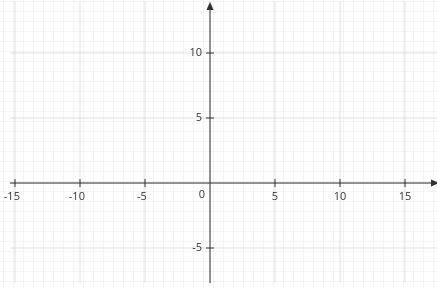
\includegraphics[scale=0.5]{assets/rafael/img25.png}
    \end{figure}
    Um ponto no plano cartesiano é formado pela ligação de dois pontos por retas paralelas aos eixo, e a intersecção aos eixos coordenados, como mostra a figura
    \begin{figure}[H]
        \centering
        \caption{Ponto $(5,10)$ no plano cartesiano}
        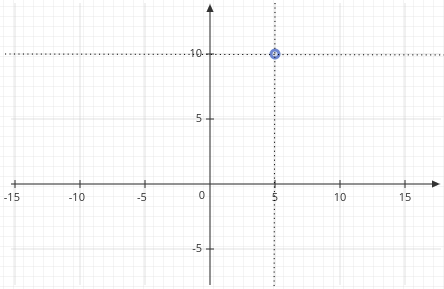
\includegraphics[scale=0.5]{assets/rafael/img26.png}
    \end{figure}

    Na figura temos a representação do ponto $(5,10)$, o valor 5 diz respeito ao valor no eixo x, e o valor 10 ao valor
    \subsection{Quadrantes do plano cartesiano}
    Os pontos, ou par ordenado, do plano cartesiano não pertencem ao eixos coordenados, e este é divido em quatro regiões onde pos pontos estão definidos:
    \begin{enumerate}
        \item Se $x \ge 0$ e $y \ge 0$, o ponto pertente ao primeiro quadrante, formalmente como

              $Q_1 = \{ (x,y)| x,y \ge 0 \}$
        \item Se $x \le $ e $ y \ge 0 $, o ponto pertence ao segundo quadrante, formalmente como

              $Q_2 = \{  (x,y) | x \le 0, y \ge 0 \}$

        \item Se $x \le $ e $ y \le 0 $, o ponto pertence ao terceiro quadrante, formalmente como

              $Q_3 = \{  (x,y) | x , y \le 0 \}$

        \item Se $x \ge $ e $ y \le 0 $, o ponto pertence ao quarto quadrante, formalmente como

              $Q_4 = \{  (x,y) | x \ge 0 ,y \le 0 \}$
    \end{enumerate}

    A figura abaixo mostra a construção do plano cartesiano
    \begin{figure}[H]
        \centering
        \caption{quadrantes do plano cartesiano}
        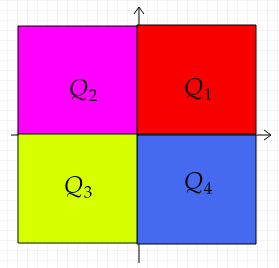
\includegraphics[scale=0.5]{assets/rafael/img28.png}
    \end{figure}
    Em cada quadrante temos a seguinte configuração dos sinais no plano cartesiano:
    \begin{figure}[H]
        \caption{Sinais no plano cartesiano}
        \centering
        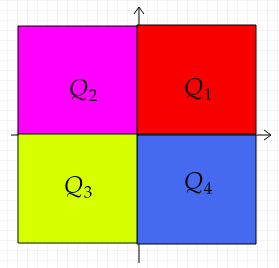
\includegraphics[scale=0.5]{assets/rafael/img28.png}
    \end{figure}

    A desiguldade triangular temos
    \subsection{Distância entre dois pontos e desiguladade triangular}


    A distância entre dois pontos, $A = (x_1,y_1)$ e $B = (x_2,y_2)$, no gráfico :


    \tikzset{every picture/.style={line width=0.75pt}} %set default line width to 0.75pt        

    \begin{tikzpicture}[x=0.75pt,y=0.75pt,yscale=-1,xscale=1]
        %uncomment if require: \path (0,4782); %set diagram left start at 0, and has height of 4782

        %Shape: Axis 2D [id:dp43431694301350077] 
        \draw  (11,225.36) -- (349.87,225.36)(143.16,18.53) -- (143.16,314) (342.87,220.36) -- (349.87,225.36) -- (342.87,230.36) (138.16,25.53) -- (143.16,18.53) -- (148.16,25.53)  ;
        %Straight Lines [id:da23706868787426827] 
        \draw    (173.75,189.23) -- (319.4,189.23) ;
        %Straight Lines [id:da2604371437830604] 
        \draw    (318.66,80.05) -- (319.4,189.23) ;
        %Straight Lines [id:da0096182706305048] 
        \draw    (318.66,80.05) -- (173.75,189.23) ;
        %Straight Lines [id:da1570173055070858] 
        \draw  [dash pattern={on 0.84pt off 2.51pt}]  (173.75,13.33) -- (173,298.4) ;
        %Straight Lines [id:da11934508201634708] 
        \draw  [dash pattern={on 0.84pt off 2.51pt}]  (343.18,189.23) -- (28.84,188.36) ;
        %Straight Lines [id:da7379908261055956] 
        \draw  [dash pattern={on 0.84pt off 2.51pt}]  (318.66,9) -- (319.22,91.31) -- (318.66,305.34) ;
        %Straight Lines [id:da892278310694206] 
        \draw  [dash pattern={on 0.84pt off 2.51pt}]  (390,80.05) -- (14.72,79.18) ;

        % Text Node
        \draw (721,21) node    {$0$};
        % Text Node
        \draw (701,71) node    {$0$};
        % Text Node
        \draw (124.59,169.23) node [anchor=north west][inner sep=0.75pt]    {$y_{1}$};
        % Text Node
        \draw (320.94,201.72) node [anchor=north west][inner sep=0.75pt]    {$\ x_{2}$};
        % Text Node
        \draw (159.93,189.43) node [anchor=north west][inner sep=0.75pt]    {$A$};
        % Text Node
        \draw (319.35,63.79) node [anchor=north west][inner sep=0.75pt]    {$B$};
        % Text Node
        \draw (174.92,206.62) node [anchor=north west][inner sep=0.75pt]    {$x_{1}$};
        % Text Node
        \draw (119.36,62.05) node [anchor=north west][inner sep=0.75pt]    {$\ y_{2}$};
        % Text Node
        \draw (231.85,171.1) node [anchor=north west][inner sep=0.75pt]    {$x_{2} -x_{1}$};
        % Text Node
        \draw (336.22,107.3) node [anchor=north west][inner sep=0.75pt]  [rotate=-89.26]  {$y_{2} -y_{1}$};


    \end{tikzpicture}

    Pelo teorema de pitágoras, a hipotenusa que liga os dois pontos é distância entre eles:

    $d(A,B) = \sqrt{ (x_2 - x_1)^2 (y_2 - y_1)^2}$

    A desiguldade triangular é a relação entre três pontos do Plano Cartesiano, onde ligados por segmentos de reta, que formam um triângulo, onde a soma de dois de lados sempre é maior que um lado, assim podemos defirnir uma regra geral para construção de triângulos no Plano Cartesiano

    \begin{theorem}
        Três pontos ligados por segmentos de reta constituem um triângulo se a soma dois segmentos forem menores ou iguais a terceiro segmento
    \end{theorem}



    \tikzset{every picture/.style={line width=0.75pt}} %set default line width to 0.75pt        

    \begin{tikzpicture}[x=0.75pt,y=0.75pt,yscale=-1,xscale=1]
        %uncomment if require: \path (0,4782); %set diagram left start at 0, and has height of 4782

        %Shape: Axis 2D [id:dp20875736416700952] 
        \draw  (-1,120.19) -- (241.57,120.19)(115.43,2) -- (115.43,225) (234.57,115.19) -- (241.57,120.19) -- (234.57,125.19) (110.43,9) -- (115.43,2) -- (120.43,9)  ;
        %Straight Lines [id:da761114184447623] 
        \draw    (172.26,17.59) -- (245.99,85.37) ;
        %Straight Lines [id:da9512079286890684] 
        \draw    (172.26,17.59) -- (57.25,88.76) ;
        %Straight Lines [id:da2855170539423624] 
        \draw    (245.99,85.37) -- (57.25,88.76) ;

        % Text Node
        \draw (721,21) node    {$0$};
        % Text Node
        \draw (701,71) node    {$0$};
        % Text Node
        \draw (34.63,81.16) node [anchor=north west][inner sep=0.75pt]    {$A$};
        % Text Node
        \draw (248.84,79.13) node [anchor=north west][inner sep=0.75pt]    {$B$};
        % Text Node
        \draw (167.85,0.96) node [anchor=north west][inner sep=0.75pt]    {$C$};
        % Text Node
        \draw (65.59,59.61) node [anchor=north west][inner sep=0.75pt]  [rotate=-325.57]  {$d( A,C)$};
        % Text Node
        \draw (123.87,70.33) node [anchor=north west][inner sep=0.75pt]  [rotate=-357.17]  {$d( A,B)$};
        % Text Node
        \draw (202.8,20.62) node [anchor=north west][inner sep=0.75pt]  [rotate=-44.39]  {$d( B,C)$};


    \end{tikzpicture}
    Matematicamente temos:

    $d(A,B) \le d(A,C) + d(B,C)$

    \subsection{Exemplo}

    \begin{enumerate}
        \item (OBMEP) Uma das diagonais de um quadrado tem extremidades A =(1,1) e C = (3,3). Quais as coordenadas dos outros vértices:

              Seguindo a ilustração:

              \begin{figure}[H]
                  \centering
                  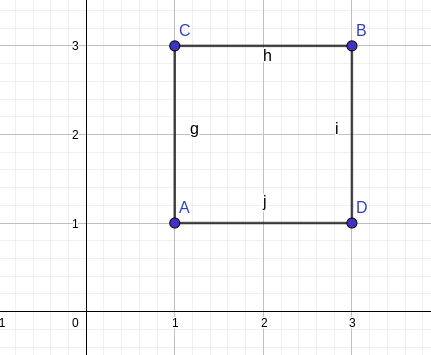
\includegraphics[scale=0.3]{assets/rafael/img29.png}
              \end{figure}

              Temos os pontos A = (1,1) e C = (3,3) a distância entre os pontos:

              $d(A,B) = \sqrt{ (x_b - x_a)^2 + (y_b - y_a)^2 }$

              $d(A,B) = \sqrt{ (3-1)^2 + (3-1)^2 } = \sqrt{(2)^2 + (2)^2}$

              $d(A,B) = \sqrt{ 4+4} = \sqrt{8} = 2 \sqrt{2}$

              Pelo teorema de pitágoras temos, que a distância da entre os pontos A e C, os demais ponto que denominamos B e D desconhecidos, sendo A,B,C e D  os pontos no plano cartesiano constituintes do quadrado

              \begin{figure}[H]
                  \centering
                  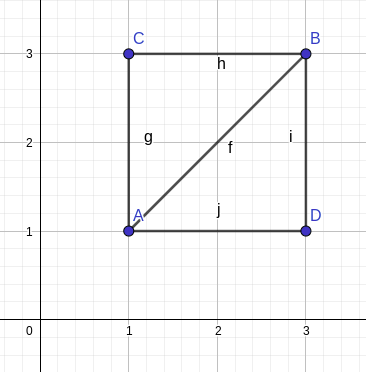
\includegraphics[scale=0.3]{assets/rafael/img30.png}
              \end{figure}

              Por teorema de pitágoras, a medida da diagonal do quadrado é $d = l\sqrt{2}$, logo a aresta do quadrado é $l = \frac{d}{\sqrt{2}}$, sendo $d = 2 \sqrt{2}$, então $l = \frac{2 \sqrt{2}}{\sqrt{2}}$, $ l = 2$
              portanto o valor dos pontos é:
              \begin{itemize}
                  \item $A = (1,1)$
                  \item $B = (x_a, y_b+2) = (1,1+2) = (1,3) $
                  \item $C = (3,3)$
                  \item $D = (x_c, y_b - 2) = (3, 3 - 2) = (3,1)$
              \end{itemize}
    \end{enumerate}
    \section{ Gráficos e Funções}

    \subsection{Funções}
    Uma função, informalmente, pode ser definida  como um conjunto de valores que podem ser 				associados por meio de uma lei com outro objeto num dado conjunto

    \begin{theorem}
        Uma função é uma lei que associa, para cada um elemento do $x$ a conjunto D, exatamente 				um elemento, conhecido como $f(x)$, em conjunto E
    \end{theorem}
    O diagrama de Venn abaixo mostra como podemos definir uma função, para cada elemento do 				conjunto de domínio é necessário um elemento no conjunto imagem.

    \begin{figure}[H]
        \centering
        \caption{Diagrama de Euler-Venn: definição de função}
        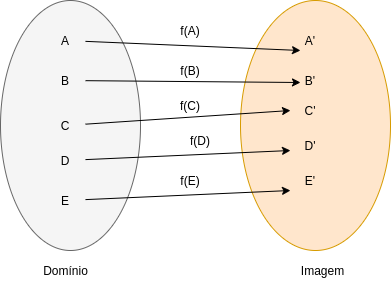
\includegraphics[scale=0.4]{assets/rafael/img.png}
    \end{figure}
    Uma Função sempre possui uma notação indicando as várias independentes, pertencentes ao 				conjunto domínio, e das variáveis dependentes
    \begin{itemize}
        \item Variáveis independentes: são as variáveis nas quais a função é avaliada, 											normalmente representada por $x$,$y$ e $z$ por exemplo
        \item Variáveis dependentes: expressam o resultado da função depois de avaliadas por 							lei, são expressas por $f(x)$ e $g(y)$ por exemplo
        \item Todo o elemento do conjunto domínio tem apenas um elemento associado no conjunto 							imagem, como mostra as figuras no modelo de diagrama de Euler-venn
    \end{itemize}

    \begin{figure}[H]
        \centering
        \caption{Diagrama de Euler-Venn: definição de função - representação válida}
        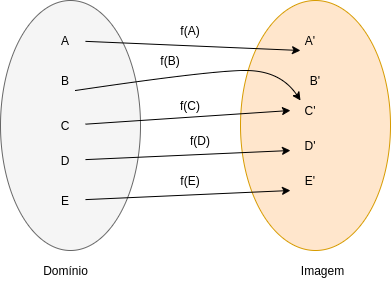
\includegraphics[scale=0.4]{assets/rafael/img1.png}
    \end{figure}


    \begin{figure}[H]
        \centering
        \caption{Diagrama de Euler-Venn: definição de função - representação inválida}
        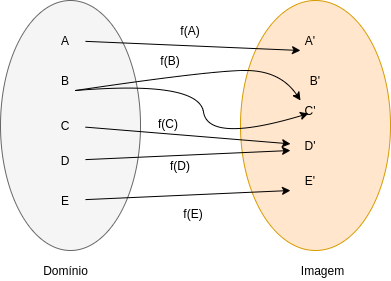
\includegraphics[scale=0.4]{assets/rafael/img2.png}
    \end{figure}
    \subsection{Formas de representação de uma função}
    \begin{enumerate}
        \item Uma função pode ter uma representação númerica de sua lei, exemplo da área de uma 						circunferência $A = \pi r^2$, de forma mais clara $A(r) = \pi r^2$
        \item Diagramas de Euler-Venn
        \item Uma função com a seguinte lei: $f(x) = \sqrt{x+2}$, tem a seguinte notação 						$ \{x \in \mathbb{R} | \forall x  \ge -2 \} $, que é lido como "x que pertence ao 						conjunto dos números reais, exceto todo valor x maior igual que -2"
        \item A função $f(x) = \cos(x^2 +3)$, que tem domínio com a representação
              $D = \{ x \in \mathbb{R} \}$, e a imagem da função $Im\{ f(x) \} =
                  \{ -1 \le x \le 1 \} $, e a leitura do conjunto imagem:  a função assume dos 						valores reais no intervalo de $\{ -1 \le x \le 1 \}$
        \item Gráficos "puramente matemáticos" como da função:
              $f(x) = \frac{ x^2 + \sin(x) }{x}$, mostrado na figura 4:
        \item Gráficos que mostram fenômenos reais, como o gráfico da figura 5, que mostra a 					evolução da média móvel de óbitos por COVID-19 até a data do dia 27 de março 2021, do 					Conselho Nacional de Secretaŕios de Saúde - CONASS


    \end{enumerate}
    \begin{figure}[H]
        \centering
        \caption{Representação gráfica da função: $f(x) = \frac{ x^2 + \sin(x) }{x}$}
        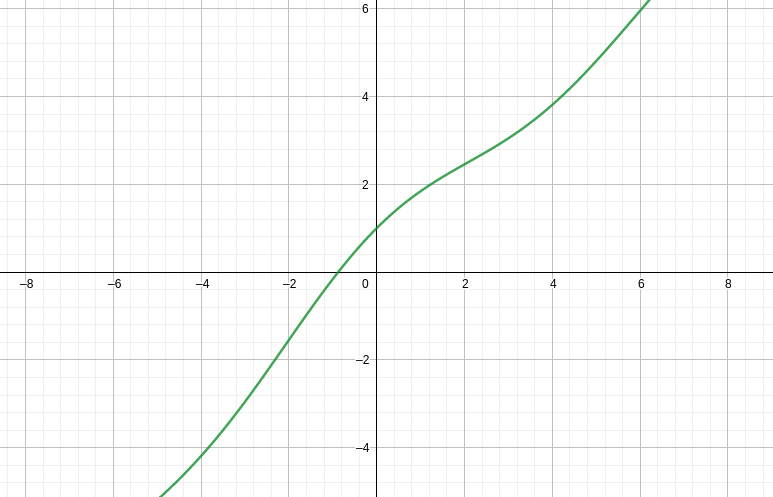
\includegraphics[scale=0.3]{assets/rafael/img3.png}
    \end{figure}

    \begin{figure}[H]
        \centering
        \caption{Evolução da média móvel de óbitos por COVID-19 - CONASS}
        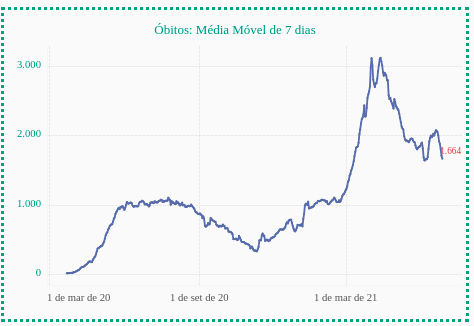
\includegraphics[scale=0.5]{assets/rafael/img4.png}
    \end{figure}


    \subsection{Domínio, Contradomínio e Imagem de uma função}

    \begin{enumerate}
        \item Domínio: o domínio de uma função é conjunto de valores possíveis que uma função pode 				assumir
        \item Contradomínio: é conjunto que reúne todas as possibilidades de imagem de uma função
        \item Imagem: conjunto possível de saída uma função segundo a lei de formação da função
    \end{enumerate}
    Como segue o segue o exemplo:

    \begin{itemize}
        \item Seja a função $f: A \rightarrow B$ cuja a lei de formação é: $f(x) = \frac{1}{x+2}$
        \item Tomando o conjunto de valores $A = \{-3,-1,0,1,2 \}$
        \item O conjunto de saídas possíveis da função $f(x)$ sobre o conjunto A, temos então o 				seguinte conjunto $B = \{f(-3),f(-1),f(0),f(1),f(2) \}$, sendo
              $B = \Big\{ -1, \frac{1}{-2}, \frac{1}{3}, \frac{1}{4} \Big\}$
    \end{itemize}


    Pela figura temos as seguintes informações:

    \tikzset{every picture/.style={line width=0.75pt}} %set default line width to 0.75pt        

    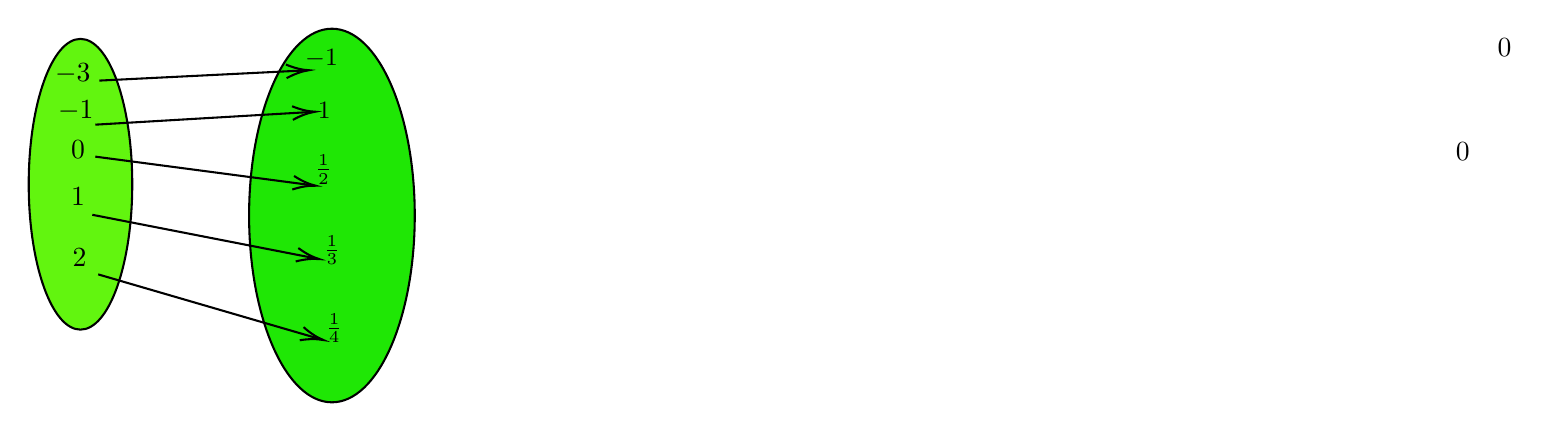
\begin{tikzpicture}[x=0.75pt,y=0.75pt,yscale=-1,xscale=1]
        %uncomment if require: \path (0,4782); %set diagram left start at 0, and has height of 4782

        %Shape: Ellipse [id:dp8420974668974206] 
        \draw  [fill={rgb, 255:red, 98; green, 245; blue, 15 }  ,fill opacity=1 ] (10,86.94) .. controls (10,48.26) and (21.17,16.9) .. (34.94,16.9) .. controls (48.72,16.9) and (59.89,48.26) .. (59.89,86.94) .. controls (59.89,125.62) and (48.72,156.98) .. (34.94,156.98) .. controls (21.17,156.98) and (10,125.62) .. (10,86.94) -- cycle ;
        %Shape: Ellipse [id:dp46917623121511953] 
        \draw  [fill={rgb, 255:red, 31; green, 231; blue, 5 }  ,fill opacity=1 ] (116.18,102) .. controls (116.18,52.29) and (134.05,12) .. (156.09,12) .. controls (178.13,12) and (196,52.29) .. (196,102) .. controls (196,151.71) and (178.13,192) .. (156.09,192) .. controls (134.05,192) and (116.18,151.71) .. (116.18,102) -- cycle ;
        %Straight Lines [id:da10018555298484899] 
        \draw    (44,37) -- (143,32.1) ;
        \draw [shift={(145,32)}, rotate = 537.1700000000001] [color={rgb, 255:red, 0; green, 0; blue, 0 }  ][line width=0.75]    (10.93,-3.29) .. controls (6.95,-1.4) and (3.31,-0.3) .. (0,0) .. controls (3.31,0.3) and (6.95,1.4) .. (10.93,3.29)   ;
        %Straight Lines [id:da9553831866701201] 
        \draw    (42.07,58.23) -- (146,52.12) ;
        \draw [shift={(148,52)}, rotate = 536.64] [color={rgb, 255:red, 0; green, 0; blue, 0 }  ][line width=0.75]    (10.93,-3.29) .. controls (6.95,-1.4) and (3.31,-0.3) .. (0,0) .. controls (3.31,0.3) and (6.95,1.4) .. (10.93,3.29)   ;
        %Straight Lines [id:da059591789314602295] 
        \draw    (42.07,73.63) -- (146.27,87.38) ;
        \draw [shift={(148.25,87.64)}, rotate = 187.52] [color={rgb, 255:red, 0; green, 0; blue, 0 }  ][line width=0.75]    (10.93,-3.29) .. controls (6.95,-1.4) and (3.31,-0.3) .. (0,0) .. controls (3.31,0.3) and (6.95,1.4) .. (10.93,3.29)   ;
        %Straight Lines [id:da10503442565965981] 
        \draw    (40.64,101.65) -- (148.04,122.62) ;
        \draw [shift={(150,123)}, rotate = 191.05] [color={rgb, 255:red, 0; green, 0; blue, 0 }  ][line width=0.75]    (10.93,-3.29) .. controls (6.95,-1.4) and (3.31,-0.3) .. (0,0) .. controls (3.31,0.3) and (6.95,1.4) .. (10.93,3.29)   ;
        %Straight Lines [id:da01808487973740891] 
        \draw    (43.49,130.37) -- (150.08,161.44) ;
        \draw [shift={(152,162)}, rotate = 196.25] [color={rgb, 255:red, 0; green, 0; blue, 0 }  ][line width=0.75]    (10.93,-3.29) .. controls (6.95,-1.4) and (3.31,-0.3) .. (0,0) .. controls (3.31,0.3) and (6.95,1.4) .. (10.93,3.29)   ;

        % Text Node
        \draw (721,21) node    {$0$};
        % Text Node
        \draw (701,71) node    {$0$};
        % Text Node
        \draw (21.24,27.51) node [anchor=north west][inner sep=0.75pt]    {$-3$};
        % Text Node
        \draw (22.66,45.02) node [anchor=north west][inner sep=0.75pt]    {$-1$};
        % Text Node
        \draw (28.94,64.63) node [anchor=north west][inner sep=0.75pt]    {$0$};
        % Text Node
        \draw (28.94,87.05) node [anchor=north west][inner sep=0.75pt]    {$1$};
        % Text Node
        \draw (29.66,116.46) node [anchor=north west][inner sep=0.75pt]    {$2$};
        % Text Node
        \draw (141.67,20.51) node [anchor=north west][inner sep=0.75pt]  [font=\small]  {$-1$};
        % Text Node
        \draw (147.85,45.81) node [anchor=north west][inner sep=0.75pt]  [font=\small]  {$1$};
        % Text Node
        \draw (146.52,71.24) node [anchor=north west][inner sep=0.75pt]  [font=\small]  {$\frac{1}{2}$};
        % Text Node
        \draw (150.52,110.16) node [anchor=north west][inner sep=0.75pt]  [font=\small]  {$\frac{1}{3}$};
        % Text Node
        \draw (151.68,147.77) node [anchor=north west][inner sep=0.75pt]  [font=\small]  {$\frac{1}{4}$};


    \end{tikzpicture}

    Para o caso do diagrama:

    \begin{enumerate}
        \item Domínio é: $D_f = \{-3,-1,0,1,2 \}$, número $x = -2$ não pertence ao domínio, porque aplicado a lei de formação da função gera uma indeterminação matemática
        \item Imagem é: $Im = \{-1,1, 1/2,1/3,1/4 \}$
        \item Contradomínio: conjunto dos números reais
    \end{enumerate}
    Generalizando as informações relativas a função
    \begin{itemize}
        \item Domínio de $f(x) = \frac{1}{x+2}$,

              $D_{f} = \{( x \in \mathbb{R}) | x = 2\}$, "x" que pertence ao número dos reais, exceto x =2

        \item Imagem de $f(x) = \frac{1}{x+2}$,

              $Im = \{x \in \mathbb{R} \}$, conjunto dos números reais

        \item Contradomínio: $CD = \{x \in \mathbb{R} \}$, conjunto dos números reais
    \end{itemize}

    \subsection{Gráfico}
    Todo gráfico pode ser uma representação de uma função, num plano com dois eixos, o eixo das 			ordenadas, eixo vertical ou simplesmente eixo y, e o eixo horizontal ou simplesmente eixo x

    O gráfico cartesiano relaciona um par ordenado (x,y), e a ligação entre esses ponto se 					materializa a construção da curva, que é a representação da função




    \subsection{Função definida por partes}
    Uma função definida por partes é uma função que assume duas expressões, nesse tipo de função, o 		seu "comportamento" se altera num dado intervalo, como exempo:

    Considere a função, f(x):
    \begin{figure}[H]
        \centering
        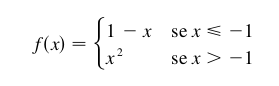
\includegraphics[scale=0.6]{assets/rafael/img6.png}
    \end{figure}
    O gráfico da função é mostrado a seguir:
    \begin{figure}[H]
        \centering
        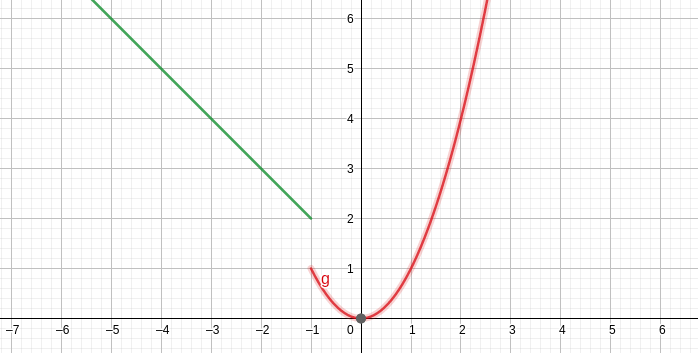
\includegraphics[scale=0.3]{assets/rafael/img5.png}
    \end{figure}
    Nesse gráfico podemos observar temos as seguintes questões:
    \begin{itemize}
        \item A função assume dois comportamentos:
              \begin{itemize}
                  \item comportamento de função linear $f(x) = 1 - x$, para todos os valores 										inferiores ou iguais -1
                  \item comportamento de função quadrática $f(x) = x^2$, para todos os valores 									maiores que -1
              \end{itemize}
        \item A função em x = -2: $-2 \le -1$, temos que a função assume o comportamento
              $f(x) = 1 -x$, logo $f(-2) = 1 - (-2)$,$f(-2) 1 + 2 = 3$
        \item A função em x = -1: $-1 \le -1$, a função mantém o comportamento pel expressão
              $f(x) = 1 - x$, logo, $f(x) = 1 - (-1) = 2$
        \item A função em x = 0: como $0 \ge -1$, logo a função assume a expressão $f(x) = x^2$ e
              $\therefore \quad f(0) = 0^2 = 0$
    \end{itemize}

    \subsection{Simetria de funções}
    Uma função é dita simétrica quando segue as seguintes propriedades:
    \begin{itemize}
        \item (x,y) = ( -x, y)
        \item (x,y) = (-x, -y)
    \end{itemize}
    Assim temos as definição de funções com simetria: funções pares e funções ímpares
    \begin{enumerate}
        \item Uma função é par quando segue a seguinte a propriedade: $f(x) = f(-x)$
        \item Uma função é ímpar quando segue a seguinte a propriedade $f(-x) = -f(x)$
    \end{enumerate}
    Fica os exemplos:
    \begin{enumerate}
        \item $	f(x) = \frac{x}{x^2 + 1} $:

              Se $f(x)$ é par, então $f(x) = f(-x)$, então $f(x) = \frac{x}{x^2 +1 }$ e
              $f(-x) = \frac{-x}{(-x)^2 +1}$, logo segue a comparação: $f(x) = f(-x)$ e portanto
              $\frac{x}{x^2 +1 } \ne \frac{ -x}{ (-x)^2 +1}$, então a função não é par

              Se $f(x)$ é impar, então $f(-x) = -f(x)$, logo $f(-x) = \frac{-x}{(-x)^2 +1}$ e
              $-f(x) = (-1) \cdot \frac{x}{x^2 +1}$, logo portanto temos que
              $\frac{-x}{(-x)^2 +1} = (-1) \cdot \frac{x}{x^2 +1} $

              $\frac{-x}{x^2 +1} = \frac{-x}{x^2 +1} $, como $f(-x) = -f(x)$, então a a função é
              ímpar

        \item $f(x) = \frac{x^2}{x^4 +1}$:

              Se $f(x)$ é par, então $f(x) = f(-x)$, sendo $f(-x) = \frac{(-x)^2}{(-x)^4 + 1}$, então

              $f(x) = f(-x)$, então $ \frac{x^2}{x^4 +1} = \frac{(-x)^2}{(-x)^4 + 1} \Rightarrow$
              $\frac{x^2}{x^4 +1} = \frac{x^2}{x^4 + 1}$, logo $f(x)$ é par

    \end{enumerate}

    \subsection{Transformações de funções}
    Transformçãoes de funções são operações aplicadas sobre uma função, no qual o  resultado pode 			ser a translação em relação ao número, rotação em torno dos eixos coordenados, expensão e 				compressão.

    Deslocamento vertical e horizontal de funções
    \begin{enumerate}
        \item $g(x) = f(x) + c$, o gráfico $f(x)$ é deslocado c unidades para cima
        \item $g(x) = f(x) - c $, o gráfico $f(x)$ é deslocado c unidades para baixo
        \item $g(x) = f(x - c) $, o gráfico $f(x)$ é deslocado c unidades para direita
        \item $g(x) = f(x + c) $, o gráfico $f(x)$ é deslocado c unidades para esquerda
    \end{enumerate}
    Na imagem a seguir vemos as operações dos items 1 e 2, na função $f(x) = x^2$
    \begin{figure}[H]
        \centering
        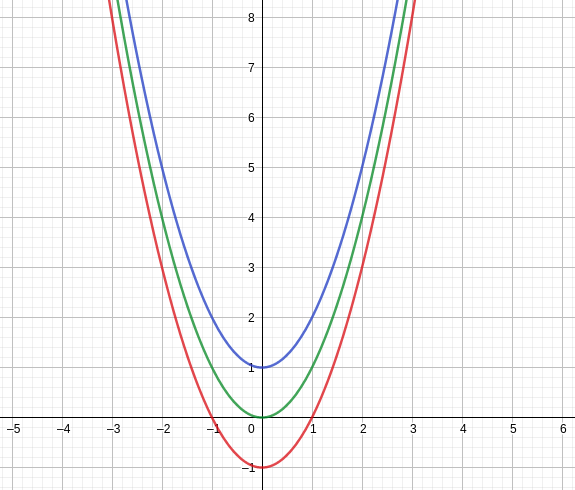
\includegraphics[scale=0.4]{assets/rafael/img7.png}
    \end{figure}
    \begin{itemize}
        \item O gráfico em verde é da "função original" $f(x) = x^2$
        \item O gráfico em azul é da função $g(x) = f(x) + 1$ que tem uma translação no eixo 							coordenado de uma unidade para cima, $g(x) = x^2 + 1 $
        \item O gráfico em vermelho é função $g(x) = f(x) - 1$ que tem uma transalação no eixo 							coordenado de uma unidade para baixo, $g(x) = x^2 -1$
    \end{itemize}
    Sobre as transformações dos itens 3 e 4, segue:
    \begin{figure}[H]
        \centering
        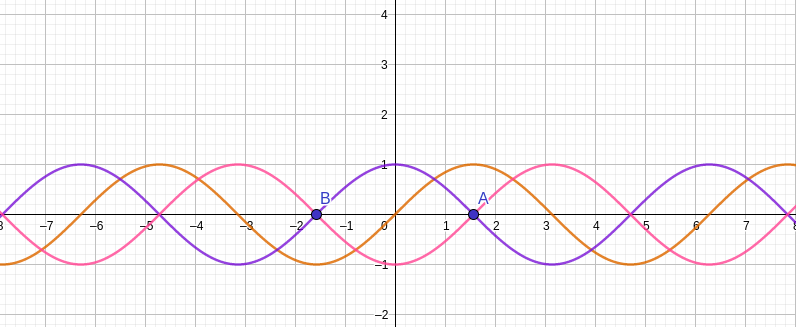
\includegraphics[scale=0.25]{assets/rafael/img8.png}
    \end{figure}
    Temos a seguinte situção:
    \begin{itemize}
        \item O gráfico em laranja representa a função $f(x) = \sin(x)$
        \item O gráfico em azul representa a função $f(x) = \sin(x + \pi/2)$ que é função seno 							desloacada $\pi/2$ unidades para a esquerda ao longo do eixo x
        \item O gráfico em rosa representa a função $f(x) = \sin(x - \pi/2)$ que é função seno 							desloacada $\pi/2$ unidades para a direita ao longo do eixo x
    \end{itemize}
    \subsection{Expansão e compressão das funções}
    Segue as seguintes propriedades de compressão e expansão de funções:

    Considere
    \begin{enumerate}
        \item $y(x) = cf(x)$, a função sofre uma expansão vertical em fator de c
        \item $y(x) = \frac{1}{c} f(x)$, a função sofre uma compressão vertical em fator de c
        \item $ y(x) = f(cx)$, compressão da função com fator de c, horizontalmente
        \item $y(x) = f(\frac{x}{c})$, expansão da função com fator de c, horizontalmente
        \item $y(x) = -f(x)$, reflexão da função em torno do eixo x
        \item $y(x)  = f(-x)$, reflexão em torno de y
    \end{enumerate}

    Para exemplificação gráfica das propriedades 1 e 2, com a função $f(x) = \cos(x)$
    \begin{figure}[H]
        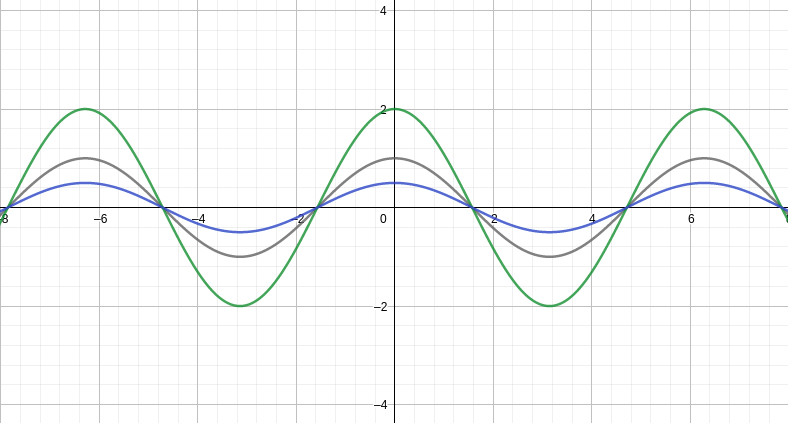
\includegraphics[scale=0.3]{assets/rafael/img10.png}
    \end{figure}

    \begin{itemize}
        \item O gráfico em cinza é da função $f(x) = \cos(x)$
        \item O gráfico em verde é da função $f(x) = 2 \cos(x)$, onde a função $\cos(x)$ tem uma 						expansão vertical em fator de c = 2
        \item O gráfico em azul é da função $f(x) = \frac{\cos(x)}{2}$, onde a função $\cos(x)$ tem 					uma compressão vertical em fator de c = 2
    \end{itemize}
    Usando a função $f(x) = \cos(x)$ para mostrar as propriedade 3 e 4, na figura a seguir:
    \begin{figure}[H]
        \centering
        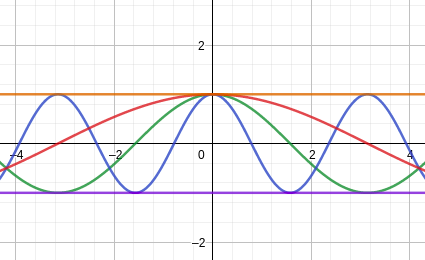
\includegraphics[scale=0.4]{assets/rafael/img9.png}
    \end{figure}
    \begin{itemize}
        \item O gráfico em verde é da função cosseno, $f(x) = \cos(x)$
        \item O gráfico em azul é da função $f(x) = \cos(2x)$, onde a função $f(x)$ sofre uma expansão 						horizontal
        \item O gráfico em vermelho é da função $f(x) = \cos \left( \frac{x}{2} \right) $
    \end{itemize}
    As propriedades 5 e 6, segue os exemplos gráficos com o polinômio: $p(x) = x^2 + x +1$
    \begin{figure}[H]
        \centering
        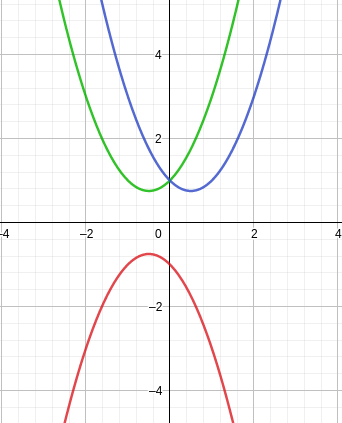
\includegraphics[scale=0.35]{assets/rafael/img11.png}
    \end{figure}
    O gráfico em verde representa o polinômio $p(x) = x^2 + x +1$, com a propriedade 5 há uma 				reflexão no eixo x, representado pelo gáfico em vermelho, e com a operação da propriedade 6 uma 		de reflexão no eixo y


    \subsection{Cominação de funções}
    Duas funções podem ser combinadas para formar novas funções, semelhante a operação númerica de 			com soma, subtração, multiplicação e divisão.

    Seja $f(x)$ e $g(x)$ duas funções, as combinações possíveis são:
    \begin{enumerate}
        \item Soma: $(f+g)(x) = f(x) + g(x)$
        \item Subtração:$(f-g)(x) = f(x) - g(x)$
        \item Multiplicação: $(f.g)(x) = f(x).g(x)$
        \item Divisão: $\left( \frac{f}{g} \right)(x)$
    \end{enumerate}

    Outra forma de combinação de funções é a operação de composição, como segue a definição:

    \begin{theorem}
        Dadas as funções $f$ e $g$, a função composta $f \circ g$ é definida por:

        $(f \circ g)(x) = f(g(x))$
    \end{theorem}
    Como exemplo temos:

    Sejam as funções $f(x) = x^2$ e $g(x) = x -3 $ a composição:
    \begin{itemize}
        \item $(f \circ g)(x) = f(g(x)) = (x-3)^2 = x^2 -6x + 9$
        \item $(g \circ f)(x) = g(f(x)) = x^2 - 3$
    \end{itemize}

    \subsection{Funções Injetoras e Inversão de funções}
    Uma função é injetora se ela nunca assume os mesmo valor duas vezes, logo $f(x_1) \ne f(x_2)$ 			sempre que $x_1 \ne x_2$

    \begin{theorem}
        O teste da reta horizontal, método gráfico de determinar se uma função é injetora, consiste em 			traçar reta horizontal, se ela não intercepta dois ponto no eixo y então a função é injetora
    \end{theorem}

    Como exemplo temos a função $f(x) = x^3$ que é uma função injetora pelo teste da reta 					horizontal, nenhuma reta horizontal "toca" dois valores igual no eixo vertical
    \begin{figure}[H]
        \centering
        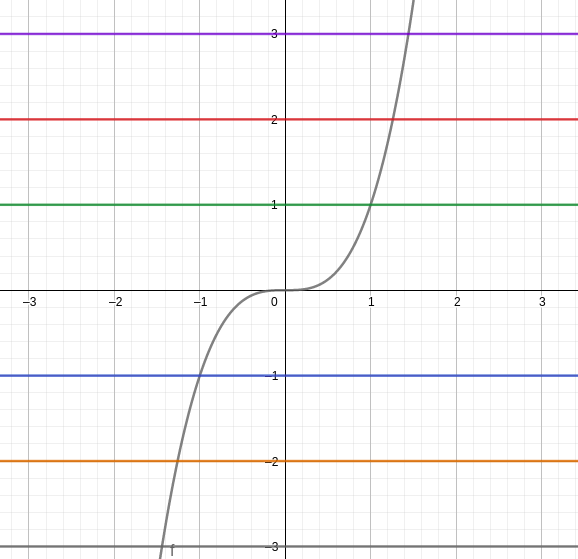
\includegraphics[scale=0.3]{assets/rafael/img37.png}
    \end{figure}

    Diferente da função $g(x) = x^2$ que não é uma função injetora pelo teste da reta horizontal

    \begin{figure}[H]
        \centering
        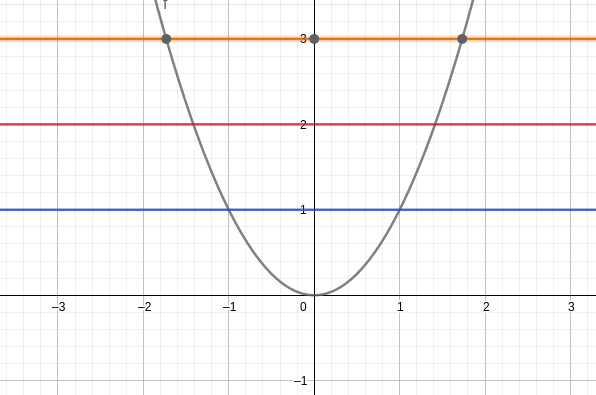
\includegraphics[scale=0.3]{assets/rafael/img38.png}
    \end{figure}

    \subsection{Inversão de funções}
    \begin{theorem}
        Uma função injetora com domínio em A e imagem em B. Então uma função inversa $f^{-1}$ tem 				domínio em B e imagem em A, e é definida por

        $f^{-1}(y) = x \Leftrightarrow f(x) = y$
    \end{theorem}

    Roteiro para inversão de funções:

    \begin{enumerate}
        \item Escreva $y = f(x)$
        \item Isole x na equação, com notação em termo de y (se possível)
        \item Na expressão de $f^{-1}$ como uma função de x, troque x por y, a expressão
    \end{enumerate}

    Como exemplo temos a seguinte função  $f(x) = x^3 +2$ seguindo o processo de 					inversão:

    $f(x) =x^3+2$ então segue:

    $y = x^3 +2 \Rightarrow x^3 +2 = y $

    $x^3 = y - 2 \Rightarrow x = \sqrt[3]{y - 2}$

    $f^{-1}(x) = \sqrt[3]{x - 2}$

    A composição de uma função com sua inversa o resultado é igual a variável da função:

    Sendo $f(x) = x^3 +2$ e $f^{-1}(x) = \sqrt[3]{x - 2}$, então temos que $f \circ f^{-1}(x)$:

    $f \circ f^{-1}(x) = (\sqrt[3]{x - 2})^3 +2$

    $f \circ f^{-1}(x) = x -2 +2$

    $f \circ f^{-1}(x) = x$
    \section{ Função Linear}
    Uma função linear é uma função que se molda com uma taxa constante, segue a a seguinte lei 				matemática: $y = f(x) = ax + b$

    Graficamente assume a geometria de uma reta, e portanto para descrever sua equação basta 				conhecer apenas dois pontos,

    A equação geral da reta é: $y - y_0 = m(x-x_0)$, onde $x_0$ e $y_0$ são os pontos conhecidos 			para se construir uma reta, e $m$ é o coeficiente de inclinação da reta

    Os exemplo deixa o tema mais claro:


    (Stweart) À medida que a temperatura do ar seco se move para cima, ele se expande e 					esfria. Se a temperatura do solo for 20ºC e temperatura a uma altitude de 1 km for de 10ºC, 			expresse a temperatura como uma função da altitude, supondo um modelo linear seja apropriado. 			Esboçe o gáfico

    Logo podemos adotar a seguinte notação: $T(h) = ah +b$, onde h é altura em quilometros, 				utilizando a equação geral da reta e desenvolvendo as operações algébricas:

    Sejam os pontos :
    \begin{equation}
        p1 = (0,20) \quad
        p2 = (1,10)
    \end{equation}
    que indicam notação cartesiana: no solo, ou altura 0km, a temperatura do é de 20ºC; com 1 km de 		altura a temperatura do ar é 20ºC

    O cáculo do coeficiente de inclinação da reta:

    $m = \frac{y-y_0}{x - x_0} = \frac{ 10 - 20}{ 1 - 0}$

    $m = \frac{-10}{1} = -10$

    Substituindo na equação geral da reta, $y - y_0 = m(x-x_0)$, temos a seguinte situação:

    $y - y_0 = m(x-x_0) \quad y - 20 = -10(x-0)$

    $y - 20 = -10x  \Rightarrow y = 20 -10x$

    O gráfico desta função pode ser obtido com os seguintes passos:
    \begin{enumerate}
        \item Tomando a função $ y = 20 -10x$, substitua x por zero: $y = 20 - 10(0) \Rightarrow
                  y = 20$, temos o par ordenado A = (0,20)
        \item Tomando a função $ y = 20 -10x$, subtitua y por zero: $0 = 20 - 10x \Rightarrow
                  x = \frac{20}{10} = 2$, temos o par ordenado B = (2,0)
        \item Marque os pontos no plano cartesiano, como mostra a figura:
              \begin{figure}[H]
                  \centering
                  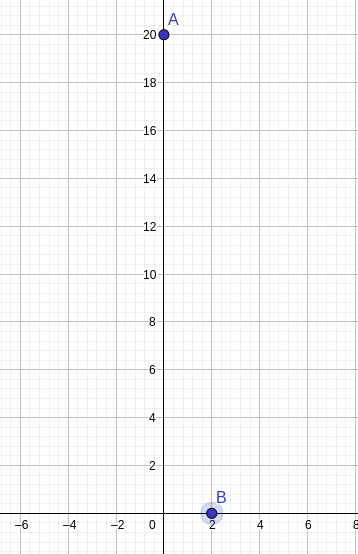
\includegraphics[scale=0.3]{assets/rafael/img12.png}
              \end{figure}
        \item Traçe uma reta ligando os dois pontos
              \begin{figure}[H]
                  \centering
                  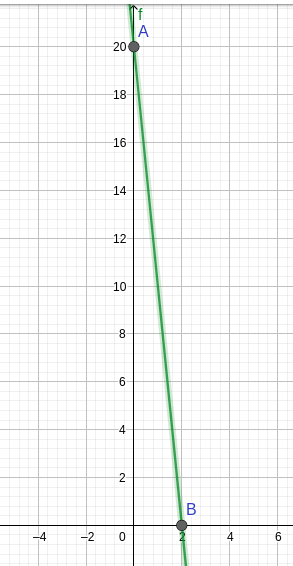
\includegraphics[scale=0.3]{assets/rafael/img13.png}
              \end{figure}
    \end{enumerate}

    Mais um exemplo :

    (UERN) Um botânico mede o crescimento de uma planta, em centímetros, todos os dias. Ligando os 			pontos, colocados por ele, num gráfico, resulta a figura abaixo
    \begin{figure}[H]
        \centering
        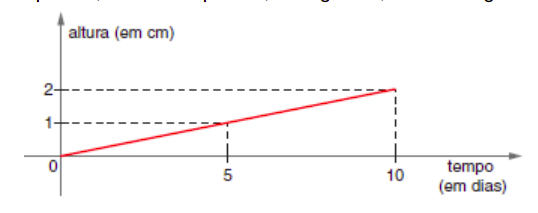
\includegraphics[scale=0.4]{assets/rafael/img15.png}
    \end{figure}
    Se mantida sempre essa relação entre tempo e altura, a planta terá no trigésimo dia, uma altura 		igual a:
    \begin{enumerate}
        \item[(a)] 5
        \item[(b)] 150
        \item[(c)] 15
        \item[(d)] 30
        \item[(e)] 6
    \end{enumerate}

    Tomando os pontos $p1= (5,1)$  e $p2 = (10,2)$, calcula-se o coeficiente de inclinação da reta:
    $m = \frac{y - y_0}{x - x_0} \quad \therefore \quad m = \frac{2 - 1}{10 - 5}
        \quad \therefore \quad m = \frac{1}{5}$

    A equação geral da reta fica: $y - y_0 = m(x-x_0) \quad \therefore \quad
        y -1 =  \frac{1}{5} \left(x - 5 \right) \quad \therefore \quad y = \frac{x}{5}$

    A função que determina reta é: $y(x) = \frac{x}{5}$, sendo x o tempo em dias e y altura da 				planta, substituindo 30 que é número de dias mencionado fica: $y(30) = \frac{30}{5} = 6$

    Letra D alternativa correta

    \section{Função Quadrática}
    Uma função quadrática, ou função do segundo grau, tema seguinte estrutura: $f(x) = ax^2 + bx 			+c$, possui o formato de um parábola, que pode ter sua curvatura ou concavidade voltada para 			cima ou para baixo.
    \begin{itemize}
        \item Concavidade para cima:
              \begin{figure}[H]
                  \centering
                  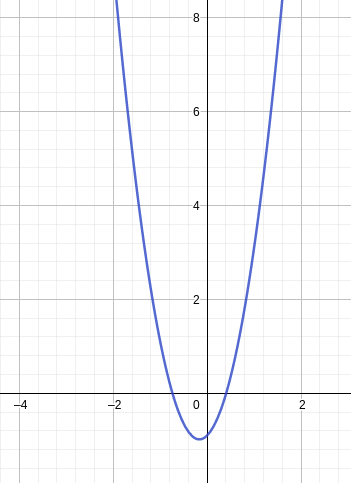
\includegraphics[scale=0.3]{assets/rafael/img16.png}
              \end{figure}
        \item Concavidade para baixo:
              \begin{figure}[H]
                  \centering
                  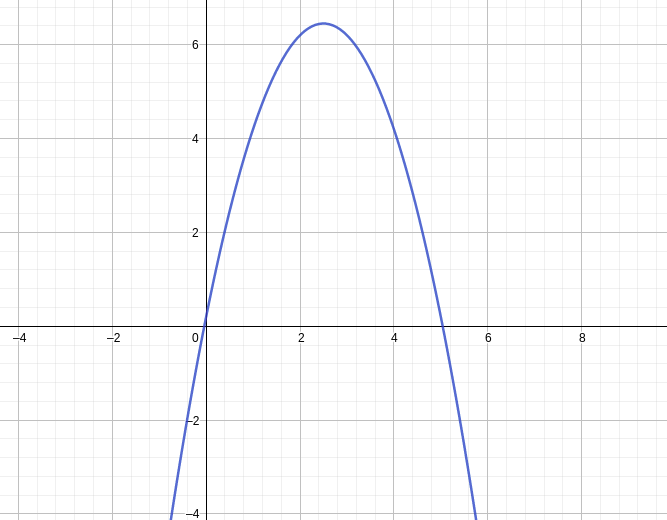
\includegraphics[scale=0.3]{assets/rafael/img17.png}
              \end{figure}
              Os principais elementos de uma função quadrática são, usados também para esboçar o seu gráfico:
              \begin{enumerate}
                  \item Raízes obtidas pelo método Báskara, se houver
                  \item Vértice
                  \item Uma vez sinalizados basta fazer o traçado de esboço
              \end{enumerate}
              \subsection{Método de Báskara}
              Método utilzado para determinar as raízes reais de uma função quadrática:
              $
                  x_{1,2} = \frac{- b \pm \sqrt{b^2 - 4ac} }{2a} \\
                  x_1 = \frac{- b + \sqrt{b^2 - 4ac} }{2a} ,
                  x_2 = \frac{- b - \sqrt{b^2 - 4ac} }{2a}
              $
              O discriminante $b^2 - 4ac$, conhecido como delta, $\Delta = b^2 - 4ac$, determina a existência 		ou não de raíz real:
              \begin{itemize}
                  \item se $\Delta = b^2 - 4ac > 0 $ então a função $f(x) = ax^2 + bx + c$ possui duas raízes 			reais distintas
                  \item se $\Delta = b^2 - 4ac = 0 $ então a função $f(x) = ax^2 + bx + c$ possui duas raízes 			reais repetidas
                  \item se $\Delta = b^2 - 4ac < 0 $  então a função $f(x) = ax^2 + bx + c$ não possui raízes 			reais
              \end{itemize}
    \end{itemize}
    Segue o exemplo:

    (UFOP) Em relação ao gráfico da função $f(x) = -x^2 + 4x -3$, pode-se afirmar :
    \begin{itemize}
        \item[(a)]é uma parábola com concavidade para cima
        \item[(b)]seu vértice é o ponto $V = (2,1)$
        \item[(c)] intercepta o eixo das abscissas em  $P = (-3,0)$ e $Q = (3,0)$
        \item[(d)]o seu eixo é o eixo das ordenadas
        \item[(e)]intercepta o eixo das ordenadas em $R = (0,3)$
    \end{itemize}
    Passos para solucionar a questão:

    Seja a função $f(x) = -x^2 + 4x -3$
    \begin{enumerate}
        \item Calcular o discriminante, delta: $\Delta = b^2 - 4ac, \quad \Delta = (4)^2 - 4.(-1).(-3)
                  \Delta = 16 - 12 = 4$
        \item Análise do valor do discriminante: como $\Delta > 0 = 4$, logo temos duas raízes reais 			distintas
        \item Cálculo do valor das raízes:
              \begin{itemize}
                  \item $x_1 = \frac{-b + \sqrt{\Delta} }{-2a}$, logo:
                        $x_1 = \frac{-4 + \sqrt{4}}{2(-1)} = \frac{ - 4 +2}{-2} = 1$
                  \item $x_2 = \frac{-b - \sqrt{\Delta} }{-2a}$
                        $x_2 = \frac{-4 - \sqrt{4}}{2(-1)} = \frac{ - 4  -2}{-2} = 3$
                        Raízes reais $x_1 = 1$ e $x_2 = 3$
              \end{itemize}
        \item Vértice: o vértice de uma parábola é média artimética de suas raízes:
              $V = \frac{x_1 +x_2}{2}$, então o ponto de vértice é $v = \frac{1+3}{3} = 4$, o valor da função 		no vétice é $f(2) = -(2^2) + 4.2 -3 = 1$
        \item Ponto de intersecção com eixo das ordenadas: substituir zero na função $f(0) = -0^2 -4.0 			-3 = -3$
        \item Com os pontos:
              \begin{itemize}
                  \item Raízes: $A = (1,0)$, $B = (3,0)$
                  \item Vértice: $C = (2,1)$
                  \item intersecção com eixo y: $D =  (0,-3)$
              \end{itemize}
              basta marcar no plano cartesiano e traçar uma parábola ligando os pontos

              Pontos no plano cartesiano:
              \begin{figure}[H]
                  \centering
                  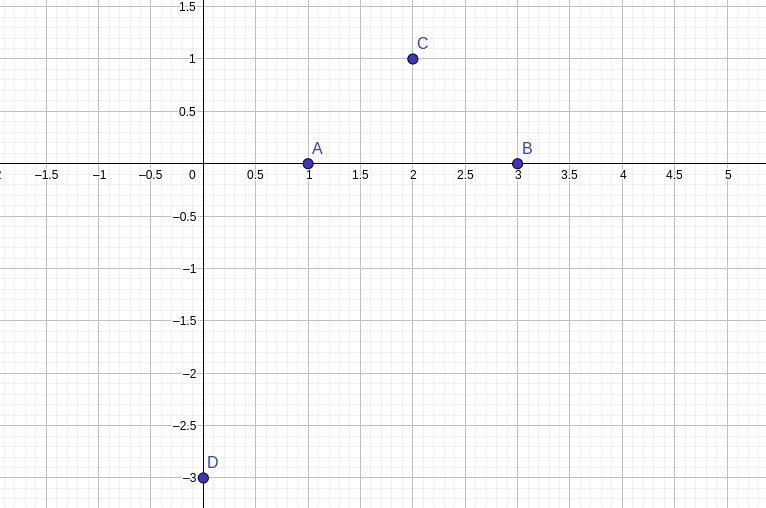
\includegraphics[scale=0.3]{assets/rafael/img18.png}
              \end{figure}
              Esboço do gráfico:
              \begin{figure}[H]
                  \centering
                  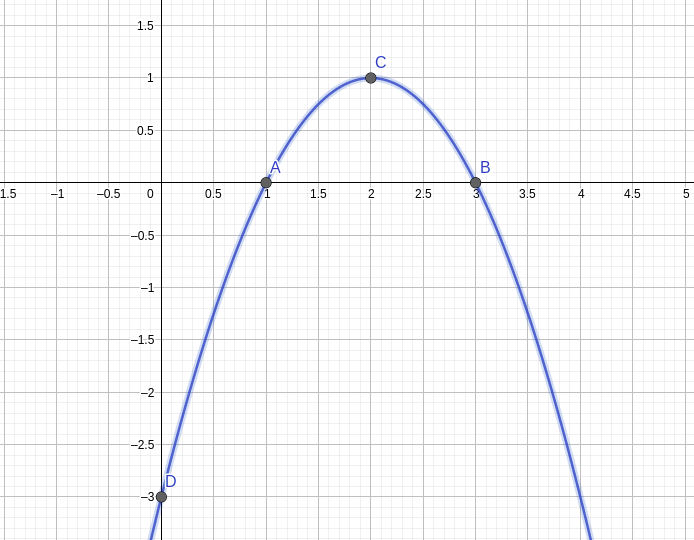
\includegraphics[scale=0.3]{assets/rafael/img19.png}
              \end{figure}

    \end{enumerate}
    Analisando as alternativas:
    \begin{itemize}
        \item[(a)] é uma parábola com concavidade para cima - Falsa, a parábola é voltada para baixo
        \item[(b)] seu vértice é o ponto $V = (2,1)$ - Correta
        \item[(c)] intercepta o eixo das abscissas em  $P = (-3,0)$ e $Q = (3,0)$ - Falsa
        \item[(d)] o seu eixo é o eixo das ordenadas -Falso, sem contexto
        \item[(e)] intercepta o eixo das ordenadas em $R = (0,3)$ - Falsa
    \end{itemize}

    Segundo exemplo:

    (FURG - RS)Um jogador de futebol se encontra a uma distância de 20 m da trave do gol 					adversário, quando chuta uma bola que vai bater exatamente sobre essa trave, de altura 2 m. Se 			a equação da trajetória da bola em relação aosistema de coordenadas indicado na figura é
    $y(x) = ax^2 + (1-2a)x$, a altura máxima atingida pela bola é:
    \begin{figure}[H]
        \centering
        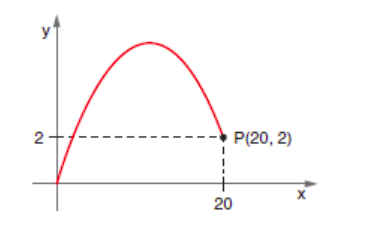
\includegraphics[scale=0.5]{assets/rafael/img20.png}
    \end{figure}
    \begin{itemize}
        \item[(a)] 6,00 m
        \item[(b)] 6,01 m
        \item[(c)] 6,05 m
        \item[(d)] 6,10 m
        \item[(e)] 6,50 m
    \end{itemize}
    Resolução:

    Pelo gráfico se conhece o ponto: $(20,2)$

    Substituindo na função: $y(x) = ax^2 + (1-2a)x$ temos: $y(20) = a(20)^2 + (1-2a)20 \quad 				\therefore	\quad 2  = a(20)^2 + (1-2a)20 $

    $2 = 400a + 20 - 40a \Rightarrow 360a + 20 = 2 \Rightarrow 360a = -18 \quad \therefore \quad
        a = \frac{-18}{ 360}$ simplificando por nove $a = \frac{-2}{ 40}$ e por dois
    $a = \frac{-1}{ 20}$

    Subustituindo o valor de a na função temos:
    $y(x) = ax^2 + (1-2a)x \Rightarrow y(x) = \frac{-1}{20} x^2 + \left( 1-2 \frac{-1}{20}
        \right)x $


    $y(x) = \frac{-x^2}{20} + \left( 1 + \frac{2}{20} \right)x$

    $y(x) = \frac{-x^2}{20} + \left(  \frac{20 +2 }{20} \right)x$

    $y(x) = \frac{-x^2}{20} + \left(  \frac{22 }{20} \right)x$

    Se substituir x = 20 na função temos:

    $y(x) = \frac{-x^2}{20} + \left(  \frac{22 }{20} \right)x$

    $y(20) = \frac{-(20)^2}{20} + \left(  \frac{22 }{20} \right)20$

    $y(20) = \frac{-400}{20} + \frac{22 . 20}{20}$

    $y(20) = \frac{-400}{20} + \frac{440}{20}$

    $y(20) = -20 + 22$

    $y(20) = 2$, valor coincidente com o apresentado pelo gráfico na questão, então é correto 				afirmar que $a = \frac{-1}{20}$

    O ponto de máximo da função de trajetório é coincidente com vértice da parábola, então podemos 			utilizar o método de báskara para determinar a solução, porém como o termo c da função é zero, 			a raíz pode ser determinada das seguinte maneira:

    $\frac{-x^2}{20} + \left(  \frac{22 }{20} \right) = 0$,
    $x \left(    \frac{-x}{20} + \frac{22}{20} \right) = 0$,
    $x = 0$ e $\left(    \frac{-x}{20} + \frac{22}{20} \right) = 0$, resolvendo a equação temos:
    $    \frac{-x}{20} + \frac{22}{20}  = 0$

    $\frac{-x}{20} = \frac{- 22}{20} \quad \therefore \quad
        20 \left( \frac{-x}{20} = \frac{- 22}{20} \right)$

    $x = 22$

    Logo as raízes são $R_1 = (0,0)$ e $R_2 = (22,0)$

    O ponto de vértice é: $v =\frac{R1 + R2}{2} =\frac{0 + 22}{2} = 11 $

    Logo $y(x) = \frac{-x^2}{20} + \frac{22x}{20}$, sendo avaliada em x = 11 dá o valor do máximo 			da trajetória

    $y(11) = \frac{-(11)^2}{20} + \frac{22.11}{20} $

    $y(11) = \frac{-121}{20} + \frac{242}{20} $

    $y(11) = -6,05 + 12,1  = 6,05 $

    A altura máxima é 6,05 m, a opção correta letra c


    \section{Funções Polinomiais}
    Como já mencionado nos tópicos anteriores, uma função é uma lei matemática que relaciona uma 			variável dois valores x e y com uma lei de formação $f(x)$, onde $(x, y = f(x))$, funções de 			primeiro $f(x) = ax + b$ e segundo grau $f(x) = ax^2 + bx + c$ são polinômios, de primeiro e 			segundo grau.

    Antes de definir o polinômio é necessário definir expressões algébricas e monômios:
    \begin{enumerate}
        \item Conjunto de operações finitas (adição, subtração, multiplicação, divisão e 						potenciação),entre variáveis nos quais os resultados fazem sentido no conjunto do números 				reais. Expressões algébricas são denotadas por letras maiúsculas, e as variáveis por letras 			minúsculas: $F = 9x^2 - \frac{8 y^4}{3}$ e $E = \frac{ \sqrt[3]{a^2 + bc^3}}{a^2 + b^2 +1 }$


        \item Monômio: é uma expressão algébrica definida pelo produto de um número real não nulo por 			um número finito de expoentes inteiros e não negativos, cujas bases são variáveis
    \end{enumerate}

    Como exemplo:
    \begin{itemize}
        \item A figura a seguir mostra um retângulo, as expressões de perímetro e área são:
              \begin{itemize}
                  \item Área: $A = x.y$
                  \item Perímetro: $ P  = 2x + 2y$
              \end{itemize}


              \tikzset{every picture/.style={line width=0.75pt}} %set default line width to 0.75pt        

              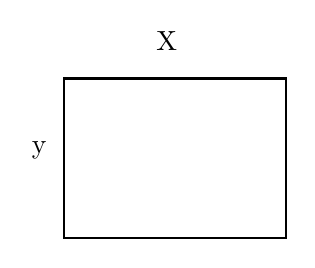
\begin{tikzpicture}[x=0.75pt,y=0.75pt,yscale=-1,xscale=1]

                  \draw   (274,61) -- (381,61) -- (381,138) -- (274,138) -- cycle ;


                  \draw (317,37) node [anchor=north west][inner sep=0.75pt]   [align=left] {X};

                  \draw (257,90) node [anchor=north west][inner sep=0.75pt]   [align=left] {y};


              \end{tikzpicture}

        \item potenciação dos seguintes monômios:
              \begin{itemize}
                  \item $\left(  \frac{1}{2} x^2y^3  \right)^4 = \frac{1}{(2)^4} x^{2.4}y^{3.4} = 								\frac{1}{16} x^8 y^{12}$
                  \item $( -\sqrt{3} a b c^3)^2 =
                            (-\sqrt{3})^2.a^2.b^2.c^{3.2} = 												(-						\sqrt{3})^2.a^2.b^2.c^6 = (-3^{1/2})^2.a^2.b^2.c^{6} = 												-3.a^2.b^2.c^6$
              \end{itemize}

    \end{itemize}
    Um polinômio é uma soma finita de monômios, por exemplo
    $p(x) = 3x^3y - 4xy^2 + \sqrt{3}xy + 8$, $p(x)$ é o polinômio na variável x, $p(x,y)$ é o 				polinômio nas variáveis x e y, e $p(x_1, x_2, \cdots, x_n)$ é polinômio nas variáveis $x_1, 			x_2, \cdots, x_n$
    O grau de um polinômio é valor do maior expoente entre os monômios

    A valoração númerica de um polinômio:

    Dado o polinômio: $E(x) = x^5 + x^4 + x^3 + x^2 + x + 1$, a valoração em x = -1 é:
    $E(-1) = (-1)^5 + (-1)^4 + (-1)^3 + (-1)^2 + (-1) + 1$,
    $E(-1) = -1 + 1 - 1 + 1 -1 +1  = 0$

    Vamos apenas tratar de polinômios de uma variável na seguinte forma:
    $p(x) = a_nx^n + a_{n-1}x^{n-1} + \cdots + a_1x + a_0$

    Exemplo (OBM):
    Determine o polinômio p(x), de grau 2, tal que: p(1) = 3, p(-2) = 9 e p(x) = p(-x):

    Um polinômio de grau 2 é dado pela forma $P(x) = ax^2 + bx + c $, usando a condição
    P(x) = P(-x):

    $P(x) = ax^2 + bx + c$

    $P(-x) = a(-x)^2 + b(-x) + c$

    $P(x) = P(-x)$

    $ax^2 + bx + c = a(-x)^2 + b(-x) + c$

    $ax^2 + bx + c = ax^2  - bx + c$

    $ax^2 + c = ax^2 + c$

    $bx = -bx \Rightarrow b = -b \Rightarrow b =0$

    Portanto a lei de formação do polinômio é $P(x) = ax^2 + c$, usando as condições  p(1) = 3, 			p(-2) - 9, logo:

    $P(x) = ax^2 + c \Rightarrow P(1) = a(1)^2 + c \Rightarrow 3 = a + c \Rightarrow a+c = 3$

    $P(x) = ax^2 + c \Rightarrow P(-2) = a(-2)^2 + c \Rightarrow 9 = 4a + c \Rightarrow 4a+c = 9$
    Fazendo uma substituição: $a + c = 3 \Rightarrow c = 3 - a \quad \therefore \quad 4a +c = 9
        4a + (3-a) = 9 \Rightarrow 4a +3 -a = 9 \Rightarrow 3a = 6 \Rightarrow a = \frac{6}{3}  = 2$

    E então temos a = 2, logo $a+c = 3 \Rightarrow 2 + c = 3 \Rightarrow c = 3 - 2 = 1$ logo com as 		constantes a = 2 e c = 1, e a lei de formação: $P(x) = 2x^2 + 1$

    \subsection{Soma, Subtração e multiplicação}
    \begin{enumerate}
        \item Soma: sejam dois polinômios $P(x) = x^2 + 3x - 4$ e $Q(x) = x^2 +2$,
              $P(x) + Q(x) = (x^2 + 3x - 4) + (x^2 +2) = x^2 +3x -4 x^2 +2 = 2x^2 + 3x -2$
        \item Subtração: sejam dois polinômios $P(x) = x^2 + 3x - 4$ e $Q(x) = x^2 +2$,
              $P(x) + Q(x) = (x^2 + 3x - 4) - (x^2 +2) = x^2 + 3x - 4 - x^2 - 2 = 3x - 6$
        \item Multiplicação: sejam dois polinômios $P(x) = x^2 + 3x - 4$ e $Q(x) = x^2 +2$,
              $P(x).Q(x) = (x^2 + 3x - 4).(x^2 +2) = x^2(x^2 +2) + 3x(x^2 +2) - 4(x^2 +2) =
                  x^4 + 2x^2 + 3x^3 + 6x - 4x^2 -8 = x^4 + 3x^3 - 2x^2 + 6x - 8$
    \end{enumerate}
    \subsection{Divisão de polinômios}
    A divisão de polinômios segue o modelo de uma divisão normal, com dividendo $D(x)$, divisor 			$Q(x)$, solução $S(x)$ e resto $R(x)$, no formato de funções como mostra a imagem
    \begin{figure}[H]
        \centering
        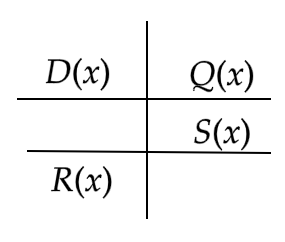
\includegraphics[scale=0.3]{assets/rafael/img21.png}
    \end{figure}

    Sejam os polinômios $A(x) = 5x^4 - 4x^2 + 3x - 1 $ e $B(x) = x^2 - 3x + 4$, logo a divisão
    $\frac{A(x)}{B(x)} = \frac{ 5x^4 - 4x^2 + 3x - 1 }{x^2 - 3x + 4} =
        \frac{ 5x^4 +0x^3 + 4x^2 + 3x - 1 }{x^2 - 3x + 4} $

    O método de divisão segue o que está a seguir:
    \begin{figure}[H]
        \centering
        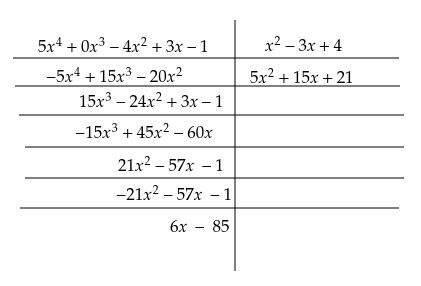
\includegraphics[scale=0.5]{assets/rafael/img22.png}
    \end{figure}
    Sendo $D(x) = 5x^4 - 4x^2 + 3x - 1$ e o divisor $Q(x) = x^2 - 3x + 4$, o quociente
    $S(x) = 5x^2 + 15x +21$ e resto $R(x) = 6x -85$
    O método consiste e equalizar o quociente com o monômio com presente no divisor, com um 				"chute" do valor para o quociente, e subtração com divisor, até que o resto seja zero ou que o 			polinômio de resto tenha um grau menor que polinômio do divisor:

    Sendo:
    $\frac{A(x)}{B(x)} = S(x) +\frac{R(x)}{D(x)}$

    \subsection{Exemplos}
    \begin{enumerate}
        \item (OBMEP) A figura abaixo representa um paralelepípedo reto-retângulo


              \begin{figure}[H]
                  \centering
                  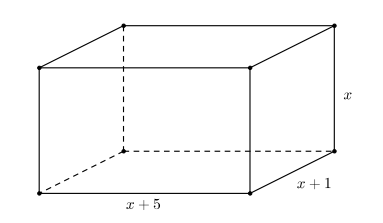
\includegraphics[scale=0.5]{assets/rafael/img24.png}
              \end{figure}
              Determine:
              \begin{enumerate}
                  \item Expressão do volume:

                        O volume de um paralelepípedo é calculado $v = a.b.c$, onde a,b e c são as 								dimensões:

                        $a = x+5, b = x+1 e c = x$

                        $v = a.b.c \therefore v = (x+5)(x+1)(x)$

                        $v = (x^2 + x + 5x +5)(x) \therefore v(x) = (x^2 +6x +5)(x)$

                        $v(x) = x^3 + 6x^2 + 5x$
                  \item o volume para x = 3
                        $v(3) = 3^3 + 6.3^2 + 5.3$

                        $v(3) = 27 + 54 + 15 = 96$
              \end{enumerate}
        \item (UFSCAR) Em relação a P(x) de terceiro grau, sabe-se que $P(-1) = 2$, $P(2) = 7$,
              $P(1) = 2$ e	$P(0) = 1$.

              \begin{enumerate}

                  \item Determine a equação reduzida da reta que passa pelo ponto que o gráfico da função $P(x)$ 			cruza o eixo y, sabendo que essa reta tem coeficiente angular numericamente igual à soma dos 			coeficientes de P(x)

                        Se $P(x)$ é um polinômio de terceiro grau, logo a lei geral de formação genérica é
                        $P(x) = ax^3 + bx^2 + cx +d$ e a equação reduzida é $y = ax +b$, a soma dos coeficientes é 				basicamente substituição de x = 1 na lei geral de formação, ainda que genérica:

                        $P(x) = ax^3 + bx^2 + cx +d$, com a avaliação em x = 1

                        $P(1) = a.1^3 + b.1^2 + c.1 +d$, como $P(1) =  2$, logo

                        $P(1) = a.1^3 + b.1^2 + c.1 +d = 2$

                        $a.1^3 + b.1^2 + c.1 +d = 2$, sendo $y = ax +b$ a equação reduzida da reta, e $a$ o coeficiente 		angular, sendo $a = 2$

                        Como o polinômio cruza o eixo y no mesmo ponto que a reta, então:

                        $P(0) = 1$, logo $y(0) = P(0)$

                        $y(0) = a.0+b \rightarrow a.0 +b = 1$

                        $b = 1 \quad \therefore \quad y = 2x + 1$

                  \item Determine P(x):

                        Com as seguintes condições (Prévia da próxima seção):
                        $P(-1) = 2, P(0) = 1, P(1) = 2, P(2) = 7$, temos

                        $P(-1) = 2$

                        $a(-1)^3 + b(-1)^2 + c(-1) + d = 2$

                        $P(0) = 0 $

                        $a.0^3 + b.0^2 + c.0 + d = 1 \quad \therefore \quad d = 1$

                        $P(1) = 2$

                        $a1^3 + b1^2 + c1 + d = 2$

                        $P(2) = 7$

                        $a2^3 + b2^2 + c2 + d = 7$

                        Com o alinhamento das equações

                        $(I) -a +b +c = 1$

                        $(II) a+b+c = 1$

                        $(III) 8a + 4b + 2c = 6$

                        Somando as equações $(I)$ e $(II)$

                        $-a +b +c = 1 +$

                        $a +b+ c = 1 \Leftrightarrow$

                        $2(b+c) = 2 \Rightarrow b+c = 1$

                        Somando as equações $(I)$ e $(III)$

                        $(III) 8a +4b + 2c = 6$

                        $(I) 8(-a+b+c = 1)$

                        $(III) 8a +4b + 2c = 6 +$

                        $(I) -8a+8b+8c = 8$

                        $12b + 10c = 14$, tomando $b+c =1$ com $b = 1 - c$

                        $12b +10(1-b) = 14$

                        $12b +10 -10b = 14 \Leftrightarrow 2b = 4$

                        $b = \frac{4}{2} = 2$

                        Sendo $b = 2$ e $c = 1 - b$ logo

                        $c = 1 - 2 = -1$

                        e $-a+b+c = 1$, então temos

                        $-a +2 - 1 = -1 \Leftrightarrow a = 2$

                        Então os coeficientes do polinômio $P(x) = ax^3 + bx^2 + cx + d$

                        $P(x) = 2x^3 +2x^2 -x +1$
              \end{enumerate}
    \end{enumerate}

    \section{Sistemas de equações do primeiro grau}
    Um sistema de equações do primeiro grau, ou sistema linear, é um conjunto de expressões 				algébricas com diferentes variáveis do primeiro grau
    \subsection{Sistema de equações com duas equações}
    $ax + by = f $

    $cx + dy = e$
    Um exemplo de como montar um sistema de equação linear

    (OBMEP)Em um sítio há somente dois tipos de animais: porcos e perus, totalizando 26 cabeças e 			72 patas. Qual a quantidade de animais de cada tipo?

    Denotando o númemero de perus por x e porcos por y, temos a seguinte equação: $x + y =26$ para 			o número de cabeças, e para o número de patas temos 2x e 2y, porque cada animal tem duas patas, 		a equação fica: $2x + 2y = 72$

    $x+y=26$

    $2x+2y = 72$

    Um sistema de equações de forma generalizada, com m equações e n linhas:

    $a_{11}x_1 + a_{12}x_2 + \cdots + a_{1n}x_n = b_1$

    $a_{21}x_1 + a_{22}x_2 + \cdots + a_{2n}x_n = b_2$

    $a_{m1}x_1 + a_{m2}x_2 + \cdots + a_{mn}x_n = b_n$

    As variáveis são indexidas por números pela quantidade finita de letras

    \subsection{Método de adição}
    Método consiste em adicionar e/ou subtrair variáveis membro a membro, de modo a manter apenas 			uma variável com solução explícita, o método permite a utilização de multiplicação de uma 				expressão algébrica por uma constante para resolução do sistema, o exemplo abaixo ajda a 				compreender melhor

    (IMPA) Um cientista M.A. Luco tem duas provetas (recipientes para líquidos) e cada uma delas 			está cheia e cada uma delas está cheia comuma substância química (plutônio ou patetônio). Se a 			capacidade dos dois recipientes somadas é 375ml e sua diferença é 75ml, quanto ele possui de 			cadasubstância, sabendo que ele possui mais plutônio que patetônio?

    Sendo x a quantidade de plutônio e y a quantidade de patetônio, pela sentença \textbf{ Se a 			capacidade dos dois recipientes somadas é 375ml} então temos a seguinte equação:

    $x + y = 375 $

    E da sentença \textbf{e sua diferença é 75ml} podemos extrair a seguinte equação:

    $x - y = 75$

    Logo temos o sistema com as seguintes equações:

    $x + y = 375 $

    $x - y = 75$

    A solução:



    \tikzset{every picture/.style={line width=0.75pt}} %set default line width to 0.75pt        

    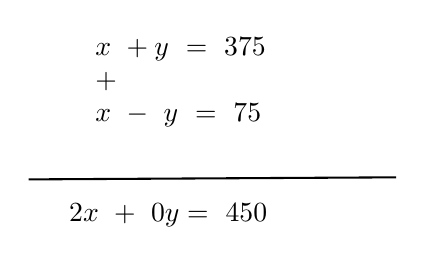
\begin{tikzpicture}[x=0.75pt,y=0.75pt,yscale=-1,xscale=1]
        %uncomment if require: \path (0,368); %set diagram left start at 0, and has height of 368

        %Straight Lines [id:da42893177853395414] 
        \draw    (183,226) -- (360,225) ;

        % Text Node
        \draw (207,153.4) node [anchor=north west][inner sep=0.75pt]    {$ \begin{array}{l}
                    x\ +y\ =\ 375 \\
                    +             \\
                    x\ -\ y\ =\ 75
                \end{array}$};
        % Text Node
        \draw (201,236.4) node [anchor=north west][inner sep=0.75pt]    {$2x\ +\ 0y=\ 450$};



    \end{tikzpicture}

    Com o resultado $2x = 450 \Rightarrow x = \frac{450}{2} = 225$, substituindo em na equação:

    $x+y = 375 \Rightarrow x = 375 - y \Rightarrow x = 375 - 225 = 150$

    \subsection{Método da substituição}
    Consiste basicamente em "resolver" uma equação e em seguida substituir a resolução em outra 			equação, como segue o exemplo a seguir:

    (IMPA). L. Santana retirou de um caixa eletrônico 330, 00 reais entre cédulas de 50, 00 reais e 		10, 00 reais num total de 17 cédulas. Qual a quantidade de cada um dos tipos de cédulas?

    Sendo x a quantidade de notas de 50 reais e y as notas de 10 reais, temos a seguinte equação:
    $50x + 10y = 330$

    A quatindade de notas é 17, logo a equação temos : $x + y = 17$, então temos:

    (I) $50x + 10y = 330$

    (II) $x + y = 17$

    A solução fica:

    Tomando a segunda equação $x + y = 17$ temos:

    $x + y = 17, \quad x = 17 - y$

    Substituindo na primeira equação:

    $50x + 10y = 330, \quad 50(17 - y) + 10y = 330, \quad 850 - 50y + 10y = 330, \quad
        -40y = 330 - 850, \quad y = \frac{520}{40} = 13$

    Utilizando a equação $x + y = 17$, sendo y = 13, então:

    $x + y = 17, \quad x + 13 = 17, \quad x = 17 - 13 = 4$

    Então são quatro notas de 50 reais e 13 notas de 10 reais

    Outro exemplo para melhor contextualização:

    (Enem): Uma companhia de seguros levantou dados sobre os carros de determinada cidade e 				constatou que são roubados, em média, 150 carros por ano. O número de carros roubados da marca 			X é o dobro do número de carros roubados da marca Y, e as marcas X e Y juntas respondem por 			cerca de 60\% dos carros roubados. O número esperado de carros roubados da marca Y é:
    \begin{itemize}
        \item[(a)] 20
        \item[(b)] 30
        \item[(c)] 40
        \item[(d)] 50
        \item[(e)] 60
    \end{itemize}

    Como a quantidade de carros roubados roubados X é o dobro de Y, logo temos a seguinte relação
    $x = 2y, \quad x - 2y = 0$

    Como a quantidade de carros roubados da soma das marcas é 60\% do total roubado, então temos:
    $60\% \times 150 = \frac{60}{100} \times 150 = \frac{6}{10} \times 150 =
        \frac{3}{5} \times 150  = \frac{3.150}{5} = 90 \quad \therefore \quad x+y = 90$

    A soma dos carros roubados das marcas x e y é 90: $x+y = 90$

    pelo método de substituição temos: $x+y = 90$, sendo $x = 2y$ segue $2y + y = 90, \quad
        3y = 90, \quad y = \frac{90}{3}, \quad y = 30$

    Como o exercício pede a quantidade de carros da marca y roubados, então como y = 30, a resposta 		correta é a letra b

    \section{Funções exponenciais}

    Uma função exponencial é uma função importante da matemática, visto que aborda os conceitos de 			crecimento populacional, e possui a seguinte estrutura geral de formação $E(x+y) = E(x)E(y)$

    Além da lei de definição $E(x+y) = E(x)E(y)$, uma função exponencial tem a variável no expoente 		e não na base, situação contrária do polinômio:
    \begin{itemize}

        \item $f(x) = a^{x}$ é uma função exponencial

        \item $f(x) = x^a$ é uma função polinomial

    \end{itemize}

    A função exponencial usa as regras de operações de potenciação, a operação de potenciação é o 			produto de um dado número pelo número de vezes do seu expoente, como os exemplos a seguir:

    \begin{enumerate}
        \item $11^2 = 11 \times 11 = 121$
        \item $17^0 = 1$ Todo número elevado a zero é igual a 1
        \item $(-4)^4 = (-4).(-4).(-4).(-4) = 256$
        \item $5^2.5^3.5^4 = 5^{2+3+4} = 5^{9} = 1953125$
        \item $\frac{3^2.3^0.3^7}{27}$, como 27 = $3^3$, $\frac{3^2.3^0.3^7}{3^3} = 3^{2+0+7}.3^{-3}
                      = 3^{9}.3^{-3} = 3^{9-3} = 3^{6} = 729$
    \end{enumerate}

    Em termos de funções exponenciais, vamos trabalhar apenas com funções com a seguinte estrtura:
    $f(x) = a^x$, onde x é uma variável do conjunto dos números reais, e a base é suas propriedades 		são:

    Seja $a \in \mathbb{R}$, a é um número fixo que pertence ao conjunto dos números reais,
    \begin{enumerate}
        \item $a^{x}.a^{y} = a^{x+y}$
        \item $a^x.b^x = (a.b)^{x}$
        \item $a^{-x} = \frac{1}{a^x}$
        \item $\frac{a^x}{a^y} = a^{x - y}$
        \item $ a^{\frac{x}{y}}  = \sqrt[y]{a^x}$
        \item $a^0 = 1$
    \end{enumerate}

    Funções esponenciais são frequentemente utilizadas em modelos populacionais com a seguinte lei 			geral de formação: $P(x) = P_0 . e^{(bx)}$, onde e é o número de Euler, e = 2,718281....


    \section{Funções logarítmicas}
    Uma função logarítmica segue as propriedades do logarítmo, e também é o operador inverso da 			potenciação, a definição de logarítmos é:

    \begin{theorem}
        Precisamente, se a > 0 e $a \ne 0$  e b > 0, o logarítmo de b na base é o expoente que 				devemos colocar na potência da base a com um resultado de b, é a solução da seguinte equação:

        $a^{y} = b$

        A solução dessa equação é: $y = \log_a b$

    \end{theorem}

    Exemplo simples:

    $\log_2 4 $ para resolver essa simples expressão temos a seguinte situação:

    Queremos determinar um número que quando elevado seja 4 tendo base 2: $2^x = 4$

    logo x = 2

    O logarítmo natural é o logarítmo na base do número de Euler = e denotado por $\log_e x = ln$

    A notação $\log$ é típica para logarítmo de base 10

    As propriedades do logarítmo são:

    \begin{enumerate}
        \item $\log_a 1 = 0$
        \item $\log_a a = 1$
        \item $a^{\log_a b} = b$
        \item $\log_a (b.c) = \log_a b + \log_a c$
        \item $\log_a \left( \frac{b}{c} \right) = \log_a b - \log_a c$
        \item $\log_a (b^k) = k.\log_a b$
        \item $\ln(e) = 1$

    \end{enumerate}


    \subsection{Exemplos com funções exponenciais e logarítmicas}

    (Escola Naval) O elemento químico Califórnio, $Cf^{251}$, emite particulas alfa, transformando-			se em Cúrio, $Cm^{247}$. Essa desintegração obedece à função exponencial $N(t) = N_0 e^{ - 				\alpha t}$ onde N(t) é a quantidade de particulas de $Cf^{251}$ no instante t em determinada 			amostra;$N_0$ é quantidade de partículas no instante inicial; e $\alpha$ é uma 							constante,chamada constante  de desintegração.Sabendo que em 898 anos a concentração de 				$Cf^{251}$ é reduzida à metade, pode-se afirmar que o tempo necessário para que a
    quantidade de $Cf^{251}$ seja apenas 25\% da quantidade inicial está entre:

    \begin{itemize}
        \item[(a)] 500 a 1000 anos
        \item[(b)] 1000 a 1500 anos
        \item[(c)] 1500 a 2000 anos
        \item[(d)] 2000 a 2500 anos
        \item[(e)] 2500 a 3000 anos
    \end{itemize}

    Resolução: primeiro precisamos determinar a constante $alpha$, em t = 898 anos a quantidade 			inicial diminui pela metade, tempo de desintegração, então temos:

    $N(898) = \frac{N_0}{2}$

    $\frac{N_0}{2} = N_0 e^{- \alpha 898}$, com temos o fator $N_0$ em ambos os lados e a equação 			fica

    $\frac{1}{2} = e^{- \alpha 898}$ aplicando o logarítmo natural em ambos os lados da equação 			temos

    $\ln \left(\frac{1}{2} \right) = \ln \left( e^{- \alpha 898} \right)$, pela propriedade dos 			logarítmos temos:

    $\ln \left(\frac{1}{2} \right) =  - \alpha 898  \therefore
        - \alpha 898 =  \left(\frac{1}{2} \right) = \alpha = \frac{-\ln(1/2)}{898} = 0,001$

    Logo a função fica $N(t) = N_0 e^{-0,001t}$, o tempo para 25\% da quantidade inicial é metade 			do tempo em relação a primeira desintegração, então a quantidade é:



    $\frac{N_0}{4} = N_0 e^{-0,001 t}, \quad \frac{1}{4} = e^{-0,001t}$

    $\ln \left( \frac{1}{4} \right) = \ln \left( e^{-0,001t} \right),
        -0,001t = \ln( 1/4), \quad t = \frac{ - \ln( 1/4)}{ 0,001}, t = 1386,294
    $
    Como t = 1386,294, então temos a letra b, como resultado correto


    (OBEMP) O processo de resfriamento de um determinado corpo descrito por
    $T(t) = T_A + \alpha.3^{\beta t}$, onde $T(t)$ é a temperatura do corpo, em grau Celsius, no 			instante t, dado em minutos, $T_A$ é a temperatura ambiente, supostamente constante, e $\alpha$
    e $\beta$ são constantes. O referido corpo foi colocado em um congelador com temperatura de 			-18ºC. Um termômetro no corpo indicou que ele atingiu 0ºC após 90 minutos e chegou a 					-16ºC após 270 minutos.
    \begin{itemize}
        \item[(a)] Encontre os valores numéricos das constantes $\alpha$ e $\beta$

              Sendo a função $T(t) = T_A + \alpha.3^{\beta t}$, tendo $T_A = -18ºC$ logo temos
              $T(t) = -18 + \alpha.3^{\beta t}$, tendo os seguintes valores de contorno $T(90) = 0$ e
              $T(270) -16$ então temos:

              $T(90) = -18 + \alpha 3^{\beta 90} \Leftrightarrow 0 = -18 + \alpha .3^{\beta 90}$

              $-18 + \alpha .3^{\beta 90} = 0 \Rightarrow \alpha.3^{\beta 90} = 18$

              $\alpha = \frac{18}{3^{\beta 90}} \Rightarrow \alpha = 18.3^{ - \beta 90}$

              Tomando $T(270) = -16$ então temos:

              $T(270) = -18 + 18.3^{ - \beta 90}.3^{- \beta 270}$

              $-16 = -18 +18.3^{\beta 180} \Rightarrow -18 +18.3^{\beta 180} = -16$

              $-18 +18.3^{\beta 180} = -16$

              $18.3^{\beta 180} = -16 +18 $

              $18.3^{\beta 180} = 2 \Rightarrow 3^{\beta 180} = \frac{2}{18} $

              $3^{\beta 180} = \frac{1}{9} \Rightarrow \log_3 3^{\beta 180} = \log_3 \left( \frac{1}{9}				\right)$

              $180 \beta \log_3 (3) = \log_3 (9^{-1})  \Rightarrow 180 \beta = -1 \log_3 (9)$

              $180 \beta = -2 \Rightarrow \beta = \frac{-2}{180} = \frac{-1}{90}$

              Tomando T(90) = 0 logo:

              $T(t) = -18 + \alpha.3^{\frac{-1}{90} t}$

              $T(90) = -18 + \alpha.3^{\frac{-90}{90} }$

              $0 = -18 + \alpha.3^{-1}$

              $-18 + \alpha.3^{-1} = 0$

              $\frac{\alpha}{3} = 18 \Rightarrow \alpha = 3.18 = 54$


              Então temos $\alpha = 54$ e $\beta = \frac{-1}{90}$

              E a função fica: $T(t) = T_A + \alpha.3^{\beta t}$
              $T(t) = -18 + 54.3^{\frac{-t}{90}}$

        \item[(b)] Determine o valor de $t$ para qual a temperatura do corpo no congelador é apenas
              $\left( \frac{2}{3} \right)$ ºC superior à temperatura no ambiente

              Logo esta temperatura: $T = \frac{2}{3} -18 $

              $T(t) = -18 + 54.3^{\frac{-t}{90}}$

              $-18 + 54.3^{\frac{-t}{90}} = -18 + \frac{2}{3}$

              $ 54.3^{\frac{-t}{90}} = \frac{2}{3}$

              $3^{\frac{-t}{90}} = \frac{2}{3.54}$

              $3^{\frac{-t}{90}} = \frac{2}{162}$

              $3^{\frac{-t}{90}} = \frac{1}{81}$

              $ \log_3 \left( 3^{\frac{-t}{90}} \right) = \log_3 \left(81^{-1} \right)$

              $\frac{-t}{90} \log_3 3 = -1 \log_3 (81)$

              $\frac{-t}{90} = -4 \Rightarrow t = 360$, tempo de 360 minutos
    \end{itemize}

    (OBMEP) Admita que um tipo de eucalipto tenha expectativa de crescimento exponencial, nos 				primeiros anos após seu plantio, modelado pela função $y(t) = a^{t-1}$, na qual $y$ representa  		altura da planta em metro, $t$ é considerado em ano, e $a$  é uma constante maior que 1. O 				gráfico representa a função $y$

    \begin{figure}[H]
        \centering
        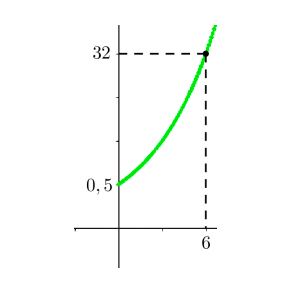
\includegraphics[scale=0.4]{assets/rafael/img23.png}
    \end{figure}
    Admita ainda que $y(0)$ fornece a altura da muda quando plantadas, e deseja-se cortar os 				eucaliptos quando as mudas crescerem $7,5m$ após o plantio. O tempo entre a plantação e corte, 			em ano, é igual a:
    \begin{itemize}
        \item[(a)] 3
        \item[(b)] 4
        \item[(c)] 6
        \item[(d)] $\log_2 7$
        \item[(e)] $\log_2 15$
    \end{itemize}
    Resolução:

    Tomando a equação $y(t) = a^{t-1}$ e a condição de $y(0) = 0,5$, logo:
    $y(0) = 0,5 \Rightarrow a^{0-1} = 0,5 \Rightarrow a^{-1} = \frac{1}{2}$

    $\frac{1}{a} = \frac{1}{2} \Rightarrow a = 2$

    Logo temos a seguinte expressão: $y = 2^{t-1}$, tendo a $y = 7,5m$, logo o tempo é:

    $y(t) = 2^{t-1} \Rightarrow 2^{t-1} = 7,5$

    $2^{t}.2^{-1} = 7,5 \Rightarrow \frac{2^{t}}{2} = 7,5$

    $2^{t} = 15 \Rightarrow t = \log_2 15$, sendo e a alternativa e

    \section{Trigonometria}

    Trigonometria é campo da matemática que estuda as relações entre comprimentos de dois lados de 			um triângulo retângulo para diferentes valores de seus ângulos, usados no estudo de 					circunferências, esferas e também no estudo de funções
    \subsection{Relações trigonométricas no triângulo retângulo}
    Um triângulo retângulo é uma figura plana com três lados, constituídos por segmentos de reta , 			com um ângulo de 90º





    \tikzset{every picture/.style={line width=0.75pt}} %set default line width to 0.75pt        

    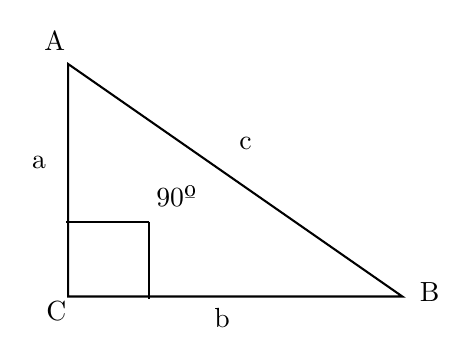
\begin{tikzpicture}[x=0.75pt,y=0.75pt,yscale=-1,xscale=1]
        %uncomment if require: \path (0,300); %set diagram left start at 0, and has height of 300

        %Shape: Right Triangle [id:dp19810997839152367] 
        \draw   (66,114) -- (227,226) -- (66,226) -- cycle ;
        %Straight Lines [id:da5995630802568936] 
        \draw    (65,190) -- (105,190) ;
        %Straight Lines [id:da9234506684523154] 
        \draw    (105,190) -- (105,227) ;

        % Text Node
        \draw (53,97) node [anchor=north west][inner sep=0.75pt]   [align=left] {A};
        % Text Node
        \draw (234,218) node [anchor=north west][inner sep=0.75pt]   [align=left] {B};
        % Text Node
        \draw (54,227) node [anchor=north west][inner sep=0.75pt]   [align=left] {C};
        % Text Node
        \draw (107,171) node [anchor=north west][inner sep=0.75pt]   [align=left] {90º};
        % Text Node
        \draw (47,157) node [anchor=north west][inner sep=0.75pt]   [align=left] {a};
        % Text Node
        \draw (135,230) node [anchor=north west][inner sep=0.75pt]   [align=left] {b};
        % Text Node
        \draw (147,148) node [anchor=north west][inner sep=0.75pt]   [align=left] {c};


    \end{tikzpicture}

    Na figura temos a representação de um triângulo retângulo, onde A,B e C são os vértices, ponto de 		encontro entre duas arestas, e as arestas que ligam dois vértices

    Todos os angulos diferente do ângulo reto são menores que 90º $\frac{\pi}{2}$ radianos, e soma dos 		ângulos de triângulo é 		igual a 180º ou a $\pi$ radianos.

    A relação fundamental para conversão de ângulos em graus para radiano é:

    $180º = \pi$, 180º é igual a $\pi$ radianos

    A figura abaixo mostra um triângulo retângulo com um ângulo de $90º$ e um ângulo $\theta$



    \tikzset{every picture/.style={line width=0.75pt}} %set default line width to 0.75pt        

    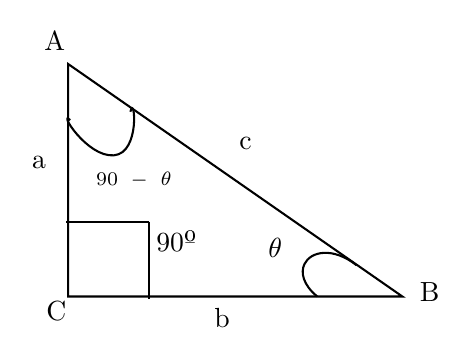
\begin{tikzpicture}[x=0.75pt,y=0.75pt,yscale=-1,xscale=1]
        %uncomment if require: \path (0,300); %set diagram left start at 0, and has height of 300

        %Shape: Right Triangle [id:dp19810997839152367] 
        \draw   (66,114) -- (227,226) -- (66,226) -- cycle ;
        %Straight Lines [id:da5995630802568936] 
        \draw    (65,190) -- (105,190) ;
        %Straight Lines [id:da9234506684523154] 
        \draw    (105,190) -- (105,227) ;
        %Curve Lines [id:da614992313810443] 
        \draw    (186,226) .. controls (179.25,220.44) and (177.86,214.56) .. (179.83,210.44) .. controls (182.82,204.18) and (193.55,201.96) .. (205,211) ;
        %Curve Lines [id:da9286805531940143] 
        \draw    (67,141) .. controls (61,136) and (75,159) .. (88,158) .. controls (101,157) and (98,128) .. (96,137) ;

        % Text Node
        \draw (53,97) node [anchor=north west][inner sep=0.75pt]   [align=left] {A};
        % Text Node
        \draw (234,218) node [anchor=north west][inner sep=0.75pt]   [align=left] {B};
        % Text Node
        \draw (54,227) node [anchor=north west][inner sep=0.75pt]   [align=left] {C};
        % Text Node
        \draw (107,193) node [anchor=north west][inner sep=0.75pt]   [align=left] {90º};
        % Text Node
        \draw (47,157) node [anchor=north west][inner sep=0.75pt]   [align=left] {a};
        % Text Node
        \draw (135,230) node [anchor=north west][inner sep=0.75pt]   [align=left] {b};
        % Text Node
        \draw (147,148) node [anchor=north west][inner sep=0.75pt]   [align=left] {c};
        % Text Node
        \draw (161,196.4) node [anchor=north west][inner sep=0.75pt]    {$\theta $};
        % Text Node
        \draw (78,164.4) node [anchor=north west][inner sep=0.75pt]  [font=\scriptsize]  {$90º\ -\ \theta $};


    \end{tikzpicture}

    Somando os ângulos $\widehat{A} = 90º$, $\widehat{B} = \theta$ e $\widehat{C} = 90 - \theta$, 			somando os ângulos temos: $\widehat{A} + \widehat{B} + \widehat{C} = 90º + \theta + (90º - \theta)=
        90º + \theta + 90º - \theta = 180º$

    A figura com a generalização:



    \tikzset{every picture/.style={line width=0.75pt}} %set default line width to 0.75pt        

    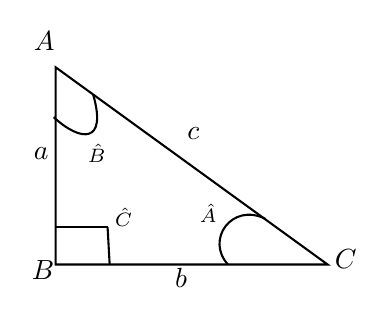
\begin{tikzpicture}[x=0.75pt,y=0.75pt,yscale=-1,xscale=1]
        %uncomment if require: \path (0,300); %set diagram left start at 0, and has height of 300

        %Shape: Right Triangle [id:dp2778932238391014] 
        \draw   (86,39) -- (217,134) -- (86,134) -- cycle ;
        %Curve Lines [id:da42478631565985303] 
        \draw    (169,134) .. controls (158,122) and (171,104) .. (187,112) ;
        %Curve Lines [id:da0357124604142427] 
        \draw    (85,63) .. controls (98,75) and (111,76) .. (104,52) ;
        %Straight Lines [id:da10309053499128273] 
        \draw    (86,116) -- (111,116) ;
        %Straight Lines [id:da17808462829740357] 
        \draw    (111,116) -- (112,134) ;

        % Text Node
        \draw (154,103.4) node [anchor=north west][inner sep=0.75pt]  [font=\scriptsize]  {$\hat{A}$};
        % Text Node
        \draw (100,74.4) node [anchor=north west][inner sep=0.75pt]  [font=\scriptsize]  {$\hat{B}$};
        % Text Node
        \draw (113,105.4) node [anchor=north west][inner sep=0.75pt]  [font=\scriptsize]  {$\hat{C}$};
        % Text Node
        \draw (74,20.4) node [anchor=north west][inner sep=0.75pt]    {$A$};
        % Text Node
        \draw (219,125.4) node [anchor=north west][inner sep=0.75pt]    {$C$};
        % Text Node
        \draw (73,130.4) node [anchor=north west][inner sep=0.75pt]    {$B$};
        % Text Node
        \draw (74,76.4) node [anchor=north west][inner sep=0.75pt]    {$a$};
        % Text Node
        \draw (142,134.4) node [anchor=north west][inner sep=0.75pt]    {$b$};
        % Text Node
        \draw (148,66.4) node [anchor=north west][inner sep=0.75pt]    {$c$};


    \end{tikzpicture}

    Um triângulo retângulo possui dois catetos e hipotenusa, maior lado do triângulo, e com isso 			podemos definir as relações trigonométricas: seno, cosseno e tangente, para determinar essas 			relações é necessário ter um ângulo de referência para a definição destas relações:





    \tikzset{every picture/.style={line width=0.75pt}} %set default line width to 0.75pt        

    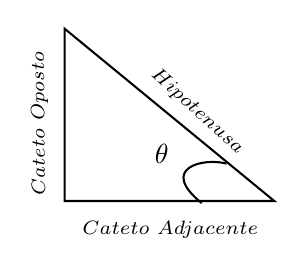
\begin{tikzpicture}[x=0.75pt,y=0.75pt,yscale=-1,xscale=1]
        %uncomment if require: \path (0,300); %set diagram left start at 0, and has height of 300

        %Shape: Right Triangle [id:dp5925596299962721] 
        \draw   (109,121) -- (210,204) -- (109,204) -- cycle ;
        %Curve Lines [id:da35593885330205777] 
        \draw    (175,205) .. controls (154,188) and (176,183) .. (187,186) ;

        % Text Node
        \draw (91.69,203.04) node [anchor=north west][inner sep=0.75pt]  [font=\scriptsize,rotate=-269.58]  {$Cateto\ Oposto$};
        % Text Node
        \draw (116,212.4) node [anchor=north west][inner sep=0.75pt]  [font=\scriptsize]  {$Cateto\ Adjacente$};
        % Text Node
        \draw (154.45,136.47) node [anchor=north west][inner sep=0.75pt]  [font=\scriptsize,rotate=-42.12]  {$Hipotenusa$};
        % Text Node
        \draw (151,175.4) node [anchor=north west][inner sep=0.75pt]    {$\theta $};


    \end{tikzpicture}

    \subsection{Definição das relações trigonométricas}
    Tomando como a figura abaixo, sendo A,B e C vértice e a,b e c arestas do triângulo de ângulo 			$\theta$:



    \tikzset{every picture/.style={line width=0.75pt}} %set default line width to 0.75pt        

    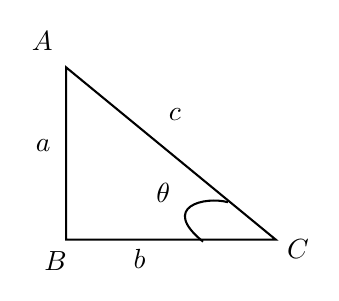
\begin{tikzpicture}[x=0.75pt,y=0.75pt,yscale=-1,xscale=1]
        %uncomment if require: \path (0,300); %set diagram left start at 0, and has height of 300

        %Shape: Right Triangle [id:dp5925596299962721] 
        \draw   (109,121) -- (210,204) -- (109,204) -- cycle ;
        %Curve Lines [id:da35593885330205777] 
        \draw    (175,205) .. controls (154,188) and (176,183) .. (187,186) ;

        % Text Node
        \draw (151,175.4) node [anchor=north west][inner sep=0.75pt]    {$\theta $};
        % Text Node
        \draw (91,102.4) node [anchor=north west][inner sep=0.75pt]    {$A$};
        % Text Node
        \draw (97,208.4) node [anchor=north west][inner sep=0.75pt]    {$B$};
        % Text Node
        \draw (214,202.4) node [anchor=north west][inner sep=0.75pt]    {$C$};
        % Text Node
        \draw (93,154.4) node [anchor=north west][inner sep=0.75pt]    {$a$};
        % Text Node
        \draw (140,207.4) node [anchor=north west][inner sep=0.75pt]    {$b$};
        % Text Node
        \draw (157,139.4) node [anchor=north west][inner sep=0.75pt]    {$c$};


    \end{tikzpicture}

    \begin{enumerate}
        \item Seno: $\sin(\theta) = \frac{ \mbox{Cateto Oposto}}{\mbox{Hipotenusa}}$
        \item Cossenho: $\cos( \theta ) = \frac{ \mbox{Cateto Adjacente}}{\mbox{Hipotenusa}}$
        \item Usando o teorema de pitágoras, com a toda dos valores de seno e cosseno do ânguo $\theta$ 		temos:

              $\sin^2(\theta) + \cos^2(\theta) =  \left( \frac{a}{c} \right)^2 + \left(  \frac{b}{c} \right)^2 =
                  \frac{a^2 + b^2}{c^2}$

              Para qualquer valor de $\theta$ temos a seguinte relação fundamental

              $\sin^2 (\theta) + \cos^2(\theta) = 1$

        \item $\sin(\theta)  = \cos \left( \frac{\pi}{2} - \theta\right)$
        \item $\cos(\theta)  = \sin \left( \frac{\pi}{2} - \theta\right)$
        \item seno da soma de dois ângulos:

              $\sin(\theta_1 + \theta_2) = \sin(\theta_1) \cos(\theta_2) + \sin( \theta_2) \cos(\theta_1)$

        \item cosseno da soma de dois ângulos:
              $\cos(\theta_1 + \theta_2) = \cos(\theta_1) \cos(\theta_2) - \sin(\theta_1) \sin(\theta_2)$

        \item Tangente de um ângulo $\theta$:

              $\tan(\theta) = \frac{\mbox{cateto oposto} }{\mbox{cateto adjacente}}$

              $\tan(\theta) = \frac{a}{b}$

        \item Cotangente de um ângulo $\theta$:

              $\cot(\theta) = \frac{b}{a}$

              $\cot(\theta) = \frac{1}{\tan(\theta)} = \frac{\mbox{cateto adjacente}}{\mbox{cateto oposto}}$

        \item Secante de um ângulo $\theta$:

              $\sec(\theta) = \frac{1}{\cos(\theta)} $

        \item Cossecante de um ângulo $\theta$

              $\csc(\theta) = \frac{1}{\sin(\theta)}$
    \end{enumerate}

    \subsection{Lei dos senos e cossenos}

    A seguinte relação:



    \tikzset{every picture/.style={line width=0.75pt}} %set default line width to 0.75pt        

    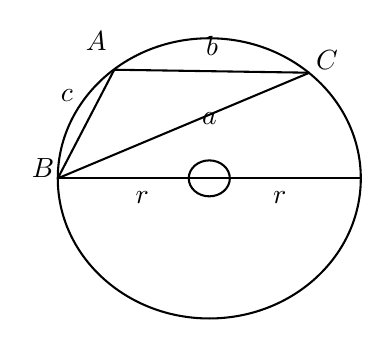
\begin{tikzpicture}[x=0.75pt,y=0.75pt,yscale=-1,xscale=1]
        %uncomment if require: \path (0,300); %set diagram left start at 0, and has height of 300

        %Flowchart: Connector [id:dp4675174331033085] 
        \draw   (187,167.5) .. controls (187,130.22) and (219.68,100) .. (260,100) .. controls (300.32,100) and (333,130.22) .. (333,167.5) .. controls (333,204.78) and (300.32,235) .. (260,235) .. controls (219.68,235) and (187,204.78) .. (187,167.5) -- cycle ;
        %Straight Lines [id:da20474778913216563] 
        \draw    (187,167.5) -- (333,167.5) ;
        %Shape: Ellipse [id:dp3998334537367554] 
        \draw   (250.1,167.5) .. controls (250.1,162.72) and (254.53,158.84) .. (260,158.84) .. controls (265.47,158.84) and (269.9,162.72) .. (269.9,167.5) .. controls (269.9,172.28) and (265.47,176.16) .. (260,176.16) .. controls (254.53,176.16) and (250.1,172.28) .. (250.1,167.5) -- cycle ;
        %Straight Lines [id:da08122516421093118] 
        \draw    (214.22,115.16) -- (308.25,116.6) ;
        %Straight Lines [id:da4045733510395637] 
        \draw    (308.25,116.6) -- (187,167.5) ;
        %Straight Lines [id:da6942970830653967] 
        \draw    (214.22,115.16) -- (187,167.5) ;

        % Text Node
        \draw (223.07,172.59) node [anchor=north west][inner sep=0.75pt]    {$r$};
        % Text Node
        \draw (289.23,172.31) node [anchor=north west][inner sep=0.75pt]    {$r$};
        % Text Node
        \draw (199,95.4) node [anchor=north west][inner sep=0.75pt]    {$A$};
        % Text Node
        \draw (173,156.4) node [anchor=north west][inner sep=0.75pt]    {$B$};
        % Text Node
        \draw (310,104.4) node [anchor=north west][inner sep=0.75pt]    {$C$};
        % Text Node
        \draw (255,134.4) node [anchor=north west][inner sep=0.75pt]    {$a$};
        % Text Node
        \draw (257,97.4) node [anchor=north west][inner sep=0.75pt]    {$b$};
        % Text Node
        \draw (187,123.4) node [anchor=north west][inner sep=0.75pt]    {$c$};


    \end{tikzpicture}

    Podemos então então inferir a lei dos senos, sendo a,b e c arestas e A, B e C vértices do 				triângulo inscrito na circunferência:

    $\frac{a}{\sin \widehat{A}} = \frac{b}{\sin \widehat{B}} = \frac{c}{\sin \widehat{C} } = 2r$

    A lei dos cossenos segue a relação do triângulo:


    \tikzset{every picture/.style={line width=0.75pt}} %set default line width to 0.75pt        

    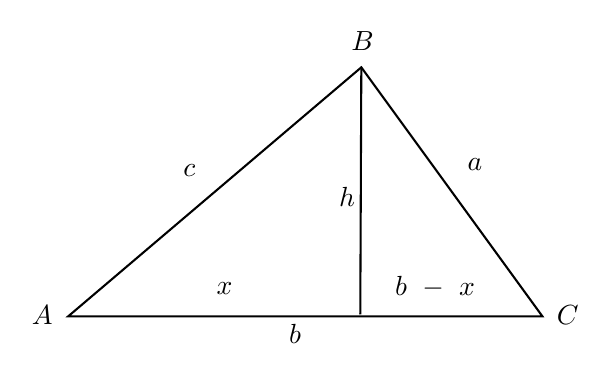
\begin{tikzpicture}[x=0.75pt,y=0.75pt,yscale=-1,xscale=1]
        %uncomment if require: \path (0,300); %set diagram left start at 0, and has height of 300

        %Flowchart: Extract [id:dp3561185957646533] 
        \draw   (194.25,64) -- (281.51,184) -- (53,184) -- cycle ;
        %Straight Lines [id:da43031858479426277] 
        \draw    (194.25,64) -- (193.75,183) ;

        % Text Node
        \draw (34,177.4) node [anchor=north west][inner sep=0.75pt]    {$A$};
        % Text Node
        \draw (188,45.4) node [anchor=north west][inner sep=0.75pt]    {$B$};
        % Text Node
        \draw (287,177.4) node [anchor=north west][inner sep=0.75pt]    {$C$};
        % Text Node
        \draw (107,109.4) node [anchor=north west][inner sep=0.75pt]    {$c$};
        % Text Node
        \draw (158,186.4) node [anchor=north west][inner sep=0.75pt]    {$b$};
        % Text Node
        \draw (244,106.4) node [anchor=north west][inner sep=0.75pt]    {$a$};
        % Text Node
        \draw (182,120.4) node [anchor=north west][inner sep=0.75pt]    {$h$};
        % Text Node
        \draw (123,166.4) node [anchor=north west][inner sep=0.75pt]    {$x$};
        % Text Node
        \draw (209,163.4) node [anchor=north west][inner sep=0.75pt]    {$b\ -\ x$};


    \end{tikzpicture}

    As relações inferidas são:

    \begin{enumerate}
        \item $x = \cos(\widehat{A}) \rightarrow $

              $ a^2 = b^2 + c^2 - 2bc \cos(\widehat{A})$

        \item $x^2 + h^2 = c^2 \rightarrow$

              $b^2 = a^2 + c^2 - 2ac \cos (\widehat{B})$

        \item $(b - x)^2 + h^2 = a^2 \Rightarrow$

              $b^2 -2bx + x^2 + h^2 = a^2 \rightarrow$

              $ c^2 = a^2 + b^2 - 2ab \cos(\widehat{C}) $
    \end{enumerate}


    \subsection{Funções Trigonométricas}

    Uma função trigonométrica é defina com a análise dos pontos localizados sobre uma circunferência, nesse contexto o sistema de coordenadas é uma circunferência de raio unitário, seguindo a linha da figura:

    \begin{figure}[H]
        \centering
        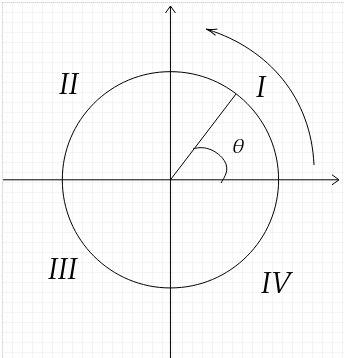
\includegraphics[scale=0.5]{assets/rafael/img31.png}
    \end{figure}

    Um ponto P presente na circunferência pode ser associado a coordenadas dos eixos coordenados, por associação temos:
    $\{ P \in C\} \rightarrow \{x \in R\}$

    $\{ P \in C\} \rightarrow \{y \in R\}$

    Sendo C a circunferência de raio unitário, e também podemos fazer a associção de um ângulo com valores presentes nos eixos coordenados

    $\{\theta \in R \} \rightarrow \{x \in R\}$

    $\{\theta \in R \} \rightarrow \{ y \in R\}$

    Assim podemos definir as funções $f(\theta) = \sin(\theta)$ e $g(\theta) = \cos(\theta)$, são funções periódiocas, onde num dado espaço a função assume mesmo valor:
    \begin{itemize}
        \item $\sin(\theta) = \sin(\theta  + 2 \pi)$
        \item $\cos(\theta) = \cos(\theta +  2 \pi)$
    \end{itemize}

    A imagem das funções seno e cosseno são:
    \begin{itemize}
        \item $-1 \le \sin(\theta) \le 1$ = $|\sin(\theta)| = 1$
        \item $-1 \le \cos(\theta) \le 1$ = $|\cos(\theta)| = 1$
    \end{itemize}

    A função tangente $f(x)  = \tan(x)$, na variável x, é definida como
    $f(x) = \tan(x) = \frac{\sin(x)}{\cos(x)}$, com domínio,
    $D_f = \{ (x \in \mathbb{R})| x \ne \frac{\pi}{2} + k \pi \}$

    A relação fundamental trigonométrica, observada pela figura:
    \begin{figure}[H]
        \centering
        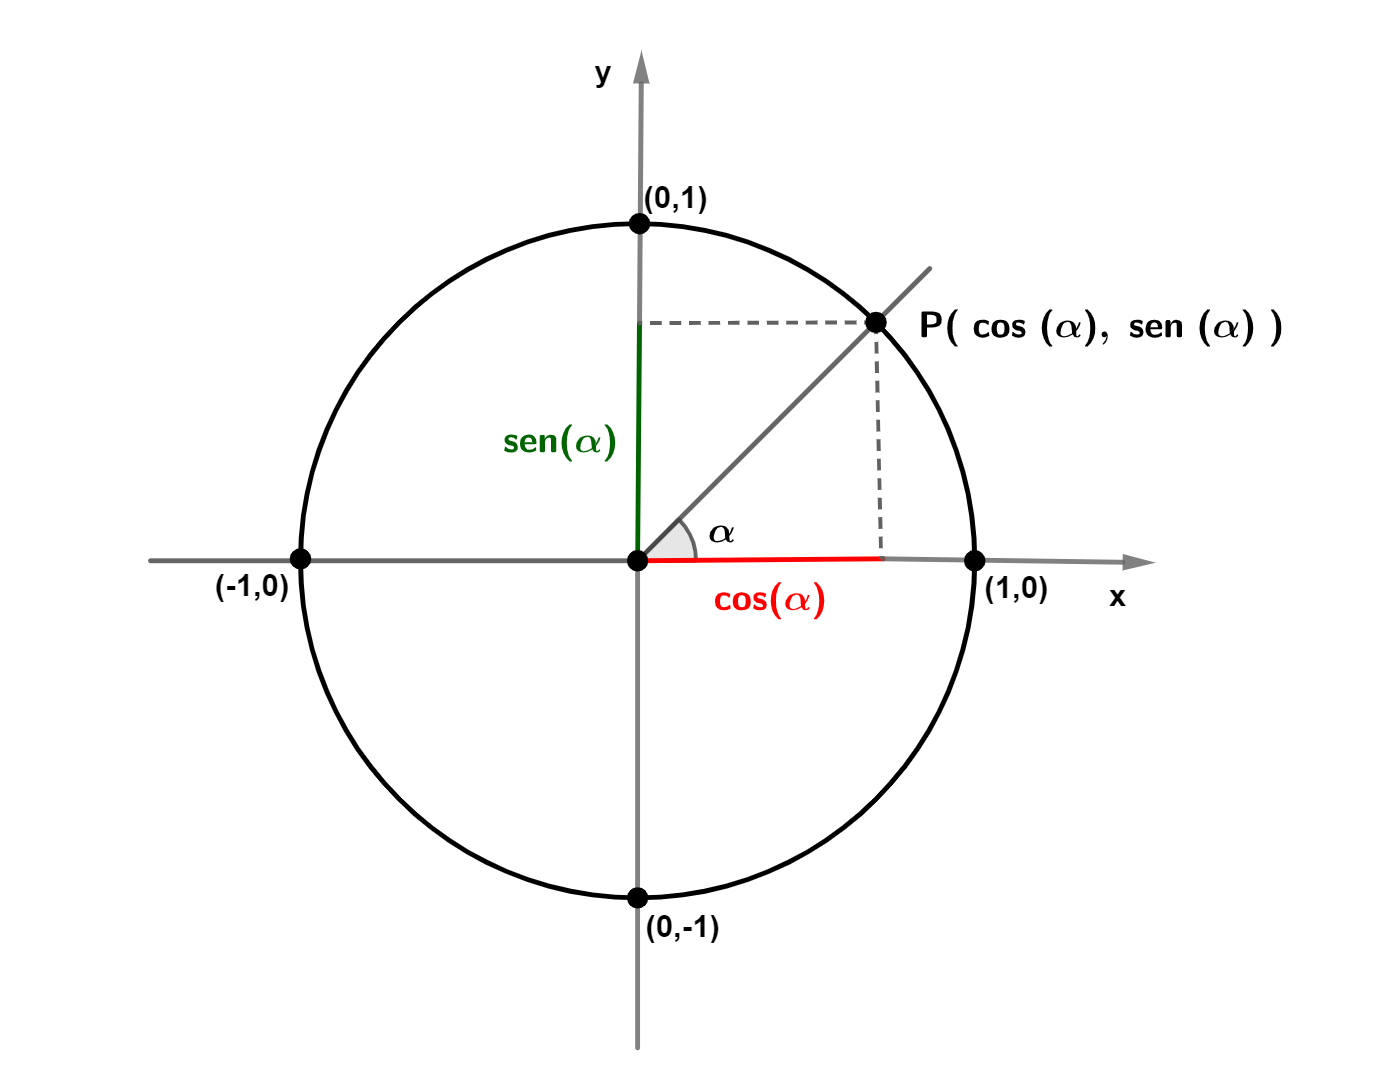
\includegraphics[scale=0.15]{assets/rafael/img32.png}
    \end{figure}
    Os catetos do triâgulo inscrito no triângulo são de medidas $\sin(\alpha)$ e $\cos(\alpha)$, por teorema de pitágoras temos a seguinte relação fundamental:

    $\sin^2(x) + \cos^2(x) = 1$ (a variálvel alfa foi substituída por x)

    O gráfico das funções trigonométricas, com avaliação nos pontos
    $\Big\{ 0, \frac{\pi}{2}, \pi, \frac{3 \pi}{2}, 2 \pi \Big\}$

    \begin{enumerate}
        \item Função seno $f(x) = \sin(x)$
              \begin{figure}[H]
                  \centering
                  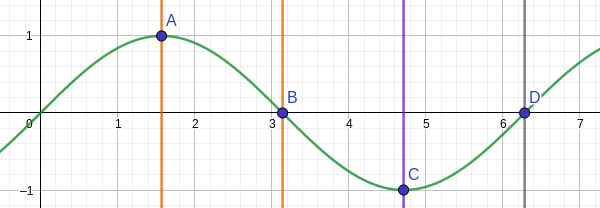
\includegraphics[scale=0.3]{assets/rafael/img33.png}
              \end{figure}
              Sendo
              \begin{itemize}
                  \item $f(0) = 0 \rightarrow \sin(0) = 0 $
                  \item $f\left(\frac{\pi}{2} \right) = 1 \rightarrow \sin \left( \frac{\pi}{2} \right) = 1 $
                  \item $f(\pi) = 0 \rightarrow \sin(\pi) = 0$
                  \item $f\left( \frac{3 \pi}{2} \right) = -1 \rightarrow \sin \left( \frac{3 \pi}{2}\right) = -1$
                  \item $f(2 \pi) = 0 \rightarrow \sin(2 \pi) = 0$
              \end{itemize}

        \item Função cosseno $f(x) = \cos(x)$
              \begin{figure}[H]
                  \centering
                  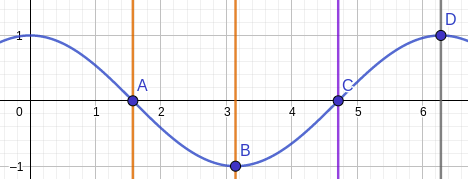
\includegraphics[scale=0.35]{assets/rafael/img34.png}
              \end{figure}
              \begin{itemize}
                  \item $f(0) = 0 \rightarrow \cos(0) = 1 $
                  \item $f\left(\frac{\pi}{2} \right) = 0 \rightarrow \cos \left( \frac{\pi}{2} \right) = 0 $
                  \item $f(\pi) = -1 \rightarrow \cos(\pi) = -1$
                  \item $f\left( \frac{3 \pi}{2} \right) = 0 \rightarrow \cos \left( \frac{3 \pi}{2}\right) = 0$
                  \item $f(2 \pi) = 1 \rightarrow \cos(2 \pi) = 0$
              \end{itemize}

        \item Função tangente $f(x) = \tan(x)$ cujo o domínio é
              $D_f = \{(x \in \mathbb{R}) | x \ne \pi /2 + k\pi \}$, nos pontos $x \ne \pi /2 + k\pi$ a função é descontínua, pela divisão por zero, uma vez que $f(x) = \tan(x) = \frac{\sin(x)}{\cos(x)}$

              \begin{figure}[H]
                  \centering
                  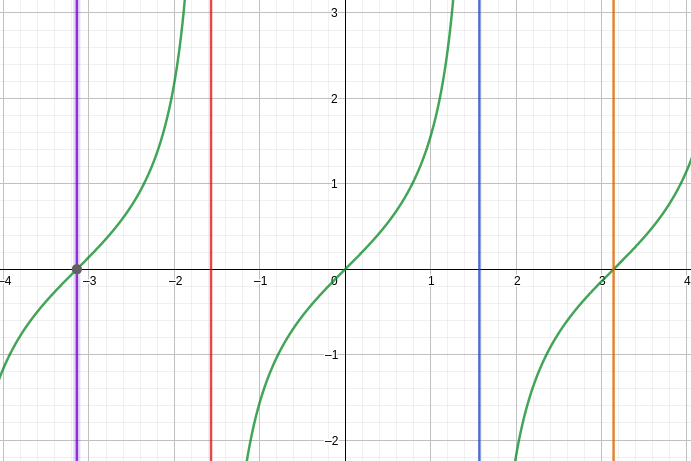
\includegraphics[scale=0.3]{assets/rafael/img35.png}
              \end{figure}

        \item Função Cotangente $f(x) = \cot(x)$, sendo definida como
              $f(x) = \cot(x) = \frac{\cos(x)}{\sin(x)}$

        \item Função Secante $f(x) = \sec(x)$, sendo definida como
              $f(x) = \frac{1}{\cos(x)} = \sec(x)$

    \end{enumerate}
    \subsection{Tabela de ângulos notáveis}
    Os ângulos notáveis com valores conhecidos das relações trigonométricas seno, cosseno e tangente, para os ângulos de 30º ou $\frac{\pi}{6}$, 45º ou $\frac{\pi}{4}$ e 60º $\frac{\pi}{3}$
    \begin{figure}[H]
        \centering
        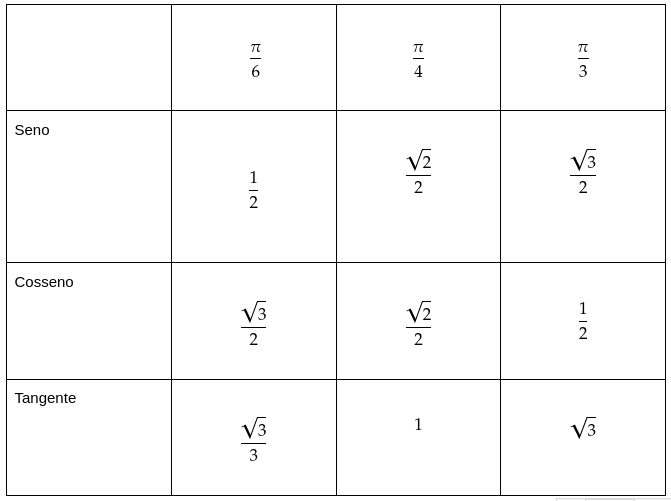
\includegraphics[scale=0.38]{assets/rafael/img36.png}
    \end{figure}

    \subsection{Funções trigonométricas inversas}

    São funções que quando compostas com sua função trigonométrica correspondente tem como "saída" o ângulo correspondente:
    \begin{enumerate}
        \item Função inversa da função seno $f(x) = \sin(x)$ é a função arcosseno $f^{-1}(x) = \arcsin(x)$
        \item Função inversa da função cosseno $f(x) = \cos(x)$ é a função arcocosseno
              $f^{-1}(x) = \arccos(x)$
        \item Função inversa da função tangente $f(x) = \tan(x)$ é a função arcotangente
              $f^{-1}(x) = \arctan(x)$
        \item Função inversa da função
    \end{enumerate}

    \subsection{Exemplos:}
    \begin{enumerate}
        \item(UFPE) Considere os triângulos PQR e PQS da figura. Se RS = 100, quanto vale PQ?

              \begin{figure}[H]
                  \centering
                  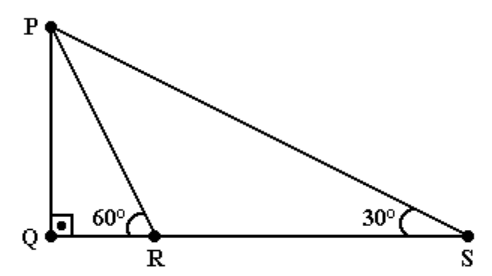
\includegraphics[scale=0.38]{assets/rafael/img39.png}
              \end{figure}
              \begin{enumerate}
                  \item $100 \sqrt{3}$
                  \item $50 \sqrt{3} $
                  \item $ 50$
                  \item $\frac{50 \sqrt{3}}{3}$
                  \item $25 \sqrt{3}$
              \end{enumerate}
              Sendo RS = 100, e medida QR desconhecida, podemos atribuir a variável x, logo $QS = 100 + x$, logo temos as seguintes relações $\tan(30º) = \frac{PQ}{QS}$ e $\tan(60º) = \frac{PQ}{QR}$, sendo 30º = $\frac{\pi}{6}$ e 60ºC = $\frac{\pi}{3}$

              Logo temos $\tan \left( \frac{\pi}{3} \right) = \frac{y}{x}$ e também temos:

              $\tan \left( \frac{\pi}{6} \right) = \frac{y}{100 +x}$

              Logo $\tan \left( \frac{\pi}{3} \right) = \frac{y}{x} \quad \therefore \quad\ \sqrt{3} = \frac{y}{x} \Rightarrow y = \sqrt{3}x$

              $\tan \left( \frac{\pi}{6} \right) = \frac{\sqrt{3} x}{100 +x} \Rightarrow
                  \frac{\sqrt{3}}{3} = \frac{\sqrt{3} x}{100 +x}$

              $\frac{1}{3} = \frac{x}{100 +x} \Rightarrow 3x = 100+X \Rightarrow3x - x = 100 \Rightarrow
                  2x = 100 \Rightarrow x = \frac{100}{2} = 50$

              Como $y = \sqrt{3} x$ então $y = 50 \sqrt{3}$, letra b resposta correta

        \item (OBMEP) Se $\sin(x) + \cos(x) = \frac{5}{6}$, então $\sin(2x)$ é igual a:
              \begin{enumerate}
                  \item $\frac{-7}{36}$
                  \item $\frac{-11}{36}$
                  \item $\frac{-13}{36}$
                  \item $\frac{-17}{36}$
                  \item $\frac{-19}{36}$
              \end{enumerate}
              Tomando a expressão $\sin(x) + \cos(x) = \frac{5}{6}$ temos a seguinte situação:

              $(\sin(x) + \cos(x))^2 = \left( \frac{5}{6} \right)^2$

              $(\sin(x) + \cos(x))\cdot(\sin(x) + \cos(x)) = \frac{25}{36}$

              $\sin^2(x) + 2 \sin(x) \cos(x) + \cos^2(x) = \frac{25}{36}$

              Sendo $\sin^2(x) + \cos^2(x) = 1$ e $\sin(2x) = \sin(x+x) = \sin(x) \cos(x) + \cos(x) \sin(x)$

              $\sin(2x) = 2 \sin(x) \cos(x)$, então a expressão fica:

              $\sin^2(x) +  \cos^2(x) + 2 \sin(x) \cos(x) = \frac{25}{36}$

              $1 + \sin(2x) = \frac{25}{36}$

              $\sin(2x) = \frac{25}{36} - 1$

              $\sin(2x) = \frac{25 - 36}{36}$

              $\sin(2x) = \frac{-11}{36}$, letra b a resposta correta

        \item (UNIRIO) Um disco voador é avistado, numa região plana, a uma certa atitude, parado no ar. Em certo instante, algo se desprende da nave e cai em queda livre, conforme mostra a figura. A que altitude se encontra esse disco voador?
              \begin{figure}[H]
                  \centering
                  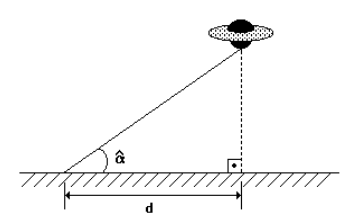
\includegraphics[scale=0.45]{assets/rafael/img40.png}
              \end{figure}
              (I) - A distância d é conhecida;

              (II) - A medida do ângulo $\alpha$ e a $\tan(\alpha)$ do mesmo ângulo são conhecida.

              Então, tem-se que:
              \begin{enumerate}
                  \item a I sozinha é suficiente para responder à pergunta, mas a II, sozinha, não
                  \item a II sozinha é suficiente para responder à pergunta, mas a I, sozinha não
                  \item I e II, juntas, são suficientes para responder à pargunta, mas nenhuma delas, sozinha, não é
                  \item ambas são, sozinhas, suficientes para responder à pergunta
                  \item a pergunta não pode ser respondida por falta de dados
              \end{enumerate}
              Resposta correta é a letra C, uma vez que a distância, seja a distância de interesse da nave, seja a distãncia vertical projetada, podem ser inferidas com os valores em questão, uma vez que podemos usar as relações trigonométricas para deduzir o valor da distância projetada e também o teorema de pitágoras para a distãncia do círculo até este ponto
    \end{enumerate}


    \bibliographystyle{plain}

    \bibliography{ref.bib}

\end{multicols*}